\documentclass[transmag]{IEEEtran}
\usepackage{latexsym}
\usepackage{graphicx}
\usepackage{amsfonts,amssymb,amsmath}
\usepackage{hyperref}
\usepackage{minted}
\usepackage{pdflscape}
\usepackage[justification=centering]{caption}
\usepackage{float}
\usepackage{hyperref}
\hypersetup{
    colorlinks=true,
    linkcolor=blue,
    filecolor=magenta,      
    urlcolor=blue,
    pdftitle={Overleaf Example},
    pdfpagemode=FullScreen,
    }

\usepackage{graphicx}
\usepackage{tabulary}
\usepackage{listings}


\usepackage[utf8]{inputenc}

\usepackage{xcolor}

\definecolor{codegreen}{rgb}{0,0.6,0}
\definecolor{codegray}{rgb}{0.5,0.5,0.5}
\definecolor{codepurple}{rgb}{0.58,0,0.82}
\definecolor{backcolour}{rgb}{0.95,0.95,0.92}


\lstdefinelanguage{JavaScript}{
  keywords={typeof, new, true, false, catch, function, return, null, catch, switch, var, if, in, while, do, else, case, break},
  keywordstyle=\color{blue}\bfseries,
  ndkeywords={class, export, boolean, throw, implements, import, this},
  ndkeywordstyle=\color{darkgray}\bfseries,
  identifierstyle=\color{black},
  sensitive=false,
  comment=[l]{//},
  morecomment=[s]{/*}{*/},
  commentstyle=\color{purple}\ttfamily,
  stringstyle=\color{red}\ttfamily,
  morestring=[b]',
  morestring=[b]",
}

\lstset{
   language=JavaScript,
   backgroundcolor=\color{white},
   extendedchars=true,
   basicstyle=\footnotesize\ttfamily,
   showstringspaces=false,
   showspaces=false,
   tabsize=2,
   breaklines=true,
   showtabs=false,
   captionpos=b
}


% \lstdefinestyle{mystyle}{
%     backgroundcolor=\color{backcolour},   
%     commentstyle=\color{codegreen},
%     keywordstyle=\color{magenta},
%     numberstyle=\tiny\color{codegray},
%     stringstyle=\color{codepurple},
%     basicstyle=\ttfamily\footnotesize,
%     breakatwhitespace=false,         
%     breaklines=true,                 
%     captionpos=b,                    
%     keepspaces=true,                 
%     numbers=left,                    
%     numbersep=5pt,                  
%     showspaces=false,                
%     showstringspaces=false,
%     showtabs=false,                  
%     tabsize=2
% }

% \lstset{style=mystyle}


\usepackage[linesnumbered,ruled,vlined]{algorithm2e}
\hypersetup{
    linkcolor=blue,
    anchorcolor=blue,
    citecolor=black,
    filecolor=blue,
    menucolor=blue,
    runcolor=blue,
    }

\def\BibTeX{{\rm B\kern-.05em{\sc i\kern-.025em b}\kern-.08em T\kern-.1667em\lower.7ex\hbox{E}\kern-.125emX}}
\markboth{COMP90024 Team 39}
{$>$ REPLACE THIS LINE WITH YOUR PAPER IDENTIFICATION NUMBER $<$}
\begin{document}

\title{Twitterlance: Fitness Analysis for Australia}

\author{Zihao Yang 1252410, Yuqi Zhang 777603, Xin Li 1029029\\
Wei Li 956833, Zihao Hu 977716}


\IEEEtitleabstractindextext{\begin{abstract}A highly scalable distributed system is developed and deployed on Melbourne Research Cloud to collect and analyse big data from Twitter. The entire deployment process is handled by Ansible tasks to enable automation and scalability. All software services are built into Docker container images for painless deployment, while the containers run in a Docker Swarm for the simplicity of scaling. The most vibrant city, sports preferences of each city, and the sport enthusiasts across six cities in Australia are identified from over 10 million tweets and the data collected from AURIN, Twitter and ESPN. The core web application, harvester, and controllers are wrapped in Django, which runs as a scalable cluster that supports parallel data collection for a better performance. All data is stored in CouchDB and processed by MapReduce in batch jobs. Spark runs as a complement to CouchDB due to the limitation of custom reduce functions on partitioned CouchDB database. Three scenarios are covered at data analysis phase, where the shows that Canberra is the most vibrant city, while running, footy, and walking are the most popular sports. Top five sports enthusiasts are identified in a rank. \end{abstract}

% 1) twitter harvest
% 2) couchdb save our data
% 3) spark couchdb Django analysis
% 4) frontend display the result
% 5) MRC docker dockerswarm HAPproxy

\begin{IEEEkeywords}
Twitterlance, Sport, Data Analysis, Scalability, Automation, Cloud, Cluster, AURIN, Twitter
\end{IEEEkeywords}}

\maketitle

\section{Introduction}

\IEEEPARstart{T}{h}is report demonstrates how we leveraged multiple applications to explore and compare the demographic pattern and sports trend in six capital cities in Australia, including Melbourne, Sydney, Perth, Brisbane, Canberra and Adelaide. 

 The performance of application developed is improved by MRC, which provides raw IT infrastructure and allows people to develop applications with low start-up cost. By running application on MRC, the data can be extracted quicker through Twitter API with parallel running design. The way to obtain topic related data is adding sport keywords as a filter for original tweets.
 
 The analysis aims to determine the most active city by comparing demographic information from AURIN platform and Twitter data, which not only examine the current tweets trends but also use historical media data to exam the active users over time when compared sports tweets in different cities, it then yields the predictive ability in observing sports trend in the future. Taking advantage of sports challenge ranks just published recently, the most hard-working fitness users are identified by summing up challenge score of mentioned sports in user's tweets. To best utilize and compare MapReduce method, we use Spark and CouchDB cluster where Django acts as a bridge. This research also demonstrates and compares the popular sports among six cities. 
 
To best present the findings of this research, our web adds multiple interactions. For example, it enables users to locate the city by inserting a city name in a Geo-search bar, as well as the popups in each circles for each city and numbers in graphs and charts. Hopefully, this analysis will not only provide users the insight about sports trends and preference  of six capital cities but also shed light on the correlation among housing price, demographic factors, education, income, unemployment and sports trends. The code on Bitbucket enables users to test and deploy a scalable solution which can be implemented on any node of unimelb MRC to store and gather partitioned Twitter data while scaling up and down automatically.

\section{Background And Related Work}
\subsection{Introduction to MRC}
Melbourne Research Cloud (MRC) is a largely Infrastructure-as-a-Service and is managed by Research Computing Services. MRC consists of almost 20000 virtual cores. It provides raw IT infrastructure and special resources like GPGPUs, private networking, load balancing, and DNS. By using MRC, researchers can access a computer quickly and build complex software with low startup costs\cite{mrc}.

\subsection{MapReduce and MPI}

At the design phase of this project, data analysis and Twitter Harvester are designed to be parallelised and distributed. Multiple parallel processing methods are evaluated, including OpenMP, MPI, and MapReduce. MapReduce and Apache Spark RDD are identified to be the best-fit data analysis method in this research. To keep the simplicity, a simple parallel model that resembles the MPI model is designed and implemented for the Twitter harvester.

Kumar and Rahman compared the performance between MPI and Apache Spark RDD in an experiment on Twitter Sentiment Analysis \cite{kumar_rahman_2017}. They developed a C++ program that runs on MPI and a Spark job implemented in Scala. Both programs are benchmarked on datasets from 200GB to 1TB. Results revealed that MPI consumes significantly less time than the Spark job because they were able to implement optimized memory allocation and task scheduling at a finely detailed level, while Spark encapsulates the program details. Another factor is that programs compiled in C++ run faster than Scala. 

Experiments from Kang, et al. \cite{kang_lee_lee_2015} compared the performance and usability of OpenMP, MPI, and MapReduce in the all-pairs-shortest-path problem. It was clear that OpenMP is only suitable for small problems, while MPI is suitable for the computation-intensive problem with moderate data size, and MapReduce has its advantage in large data size and the job does not have iterative processing. 

Twitterlance is a project that focuses on simple data analysis on a large dataset and does not require intensive computation. MapReduce is, therefore, the best choice for the data analysis model in this case. 

To parallelize the Twitter harvester, MapReduce might not be a good fit as the harvester runs in long iterative processes. The only result of the harvester is to save data to the database, which is not performance intensive. In this case, MPI or OpenMP bring excessive complexity to the system. Therefore, we designed a parallel model that divides the harvesting targets evenly across nodes via a shared database in CouchDB. 

The detailed implementations are explained in the following sections.   

\section{Software Development}

\subsection{Team Organisation}

Team 39 involves five developers. Zihao Yang was mainly responsible for the back-end development along with the system integration and deployment of the applications with Docker and Docker Swarm. Wei Li focused on Twitter harvesters, back-end data processing, and job control. Yuqi Zhang’s job was mostly Twitter harvester development and chart visualization in the user interface. Xin Li was primarily responsible for data analysis and map visualization in the user interface. Zihao Hu mainly focused on the front-end and Twitter harvesters. Apart from their major focuses, each team member also contributed to other people’s jobs upon necessity. For example, Zihao Yang optimized the front-end. Zihao Hu wrote the Ansible scripts for MRC instances creation. Yuqi Zhang and Xin Li made significant efforts in defining the research scope, as well as creating views of CouchDB a Django. Wei Li helped debug the integration. The organization and task allocation firmly ensured the team's productivity and delivery quality. 

\subsection{Development Methods}

\subsubsection{Meeting}

Meetings were held every Monday and Friday. On Monday’s meeting, members firstly show the progress done from the last week and then solve the issue encountered together. After that, weekly tasks are distributed to each member. On Friday’s meeting, we make sure each member is on the track and then solve the issue encountered together. In this project, we fully realized that the key to teamwork lies in timely and centralized communication.

\subsubsection{Trello}

Tasks are distributed and tracked with Trello by simply adding the member's name and the due date under the task. There are five parts on dashboards, ToDo, Underway, Obstacle, Complete, and Denied. On Monday’s meeting, the allocated tasks are put into the ToDo list. When there is a challenge, the member adds it into the Obstacle part, so others get notified and try to address the issue before the next meeting. If the issue is raised which we are not able to solve (due to the limitation of resources, tools, or skills), it is moved into the Denied part. After that, an alternative plan is added to the ToDo list.

\subsubsection{Remote Collaboration during COVID-19}

Completing this assignment in 5 weeks might not be an easy job, especially during COVID-19. As some members are in China, while some are in Melbourne. We are fortunate to have applications and tools provided by the University of Melbourne. All the jobs in this assignment can be completed in time through the internet. For example, our daily communication was through Slack, and tasks are tracked through Trello, all the meetings were held on ZOOM, and our team shared source code on Bitbucket. The biggest challenge for remote collaboration comes from the instability of VPN. The MRC instance is connected through the Cisco AnyConnect. However, the connection can be interrupted anytime when using Cisco AnyConnect in China \textbf{due to limited speed}. Besides, FortiClient VPN can connect to the internet but can not access MRC.

\subsubsection{Pair Programming}

During the development of complex modules such as distributed Twitter harvester job control, we exercised pair programming remotely on a voice call and IDE live to share. Compared to single engineering, coding in pairs significantly reduced the number of human mistakes. It is extremely common that a single engineer keeps thinking about a problem in a loop that does not direct to the right solution. With two people working together, it is much easier to find the best strategies out of discussions. Pair programming may provide more than double the increase of productivity as some insidious mistakes are extremely time-consuming to locate. 

\subsection{Development Process}

We followed short-term iterative development cycles where each week was a sprint. Goals and requirements were set on Monday every week. We firstly started from designing the overall architecture, drafting the analysis problem, setting up the software frameworks, and proof of concepts. In this phase, we were able to prove the feasibility of the architecture and the analysis tasks. In the next week, we began to develop the domain business logic within the chosen software framework, and the database was set up for testing. Then all software components except the load balancer were built into container images and deployed for testing. The rest of the time was consumed by engineering details. By the end of the project, we summarised time consumption for various types of tasks. The largest portion of time was spent on configuration and small adjustments on engineering. This truly showed us how long the journey is for a software product to grow up. 

\subsection{Version Control}

Git is the major version control system adopted in the development cycle. The current repository is hosted on a public \href{https://bitbucket.org/comp90024team39/comp90024-a2/src/master/}{Bitbucket workspace} (\url{https://bitbucket.org/comp90024team39/comp90024-a2/src/master/}). 

\section{Architecture and Implementation}
\begin{figure*}
\centering
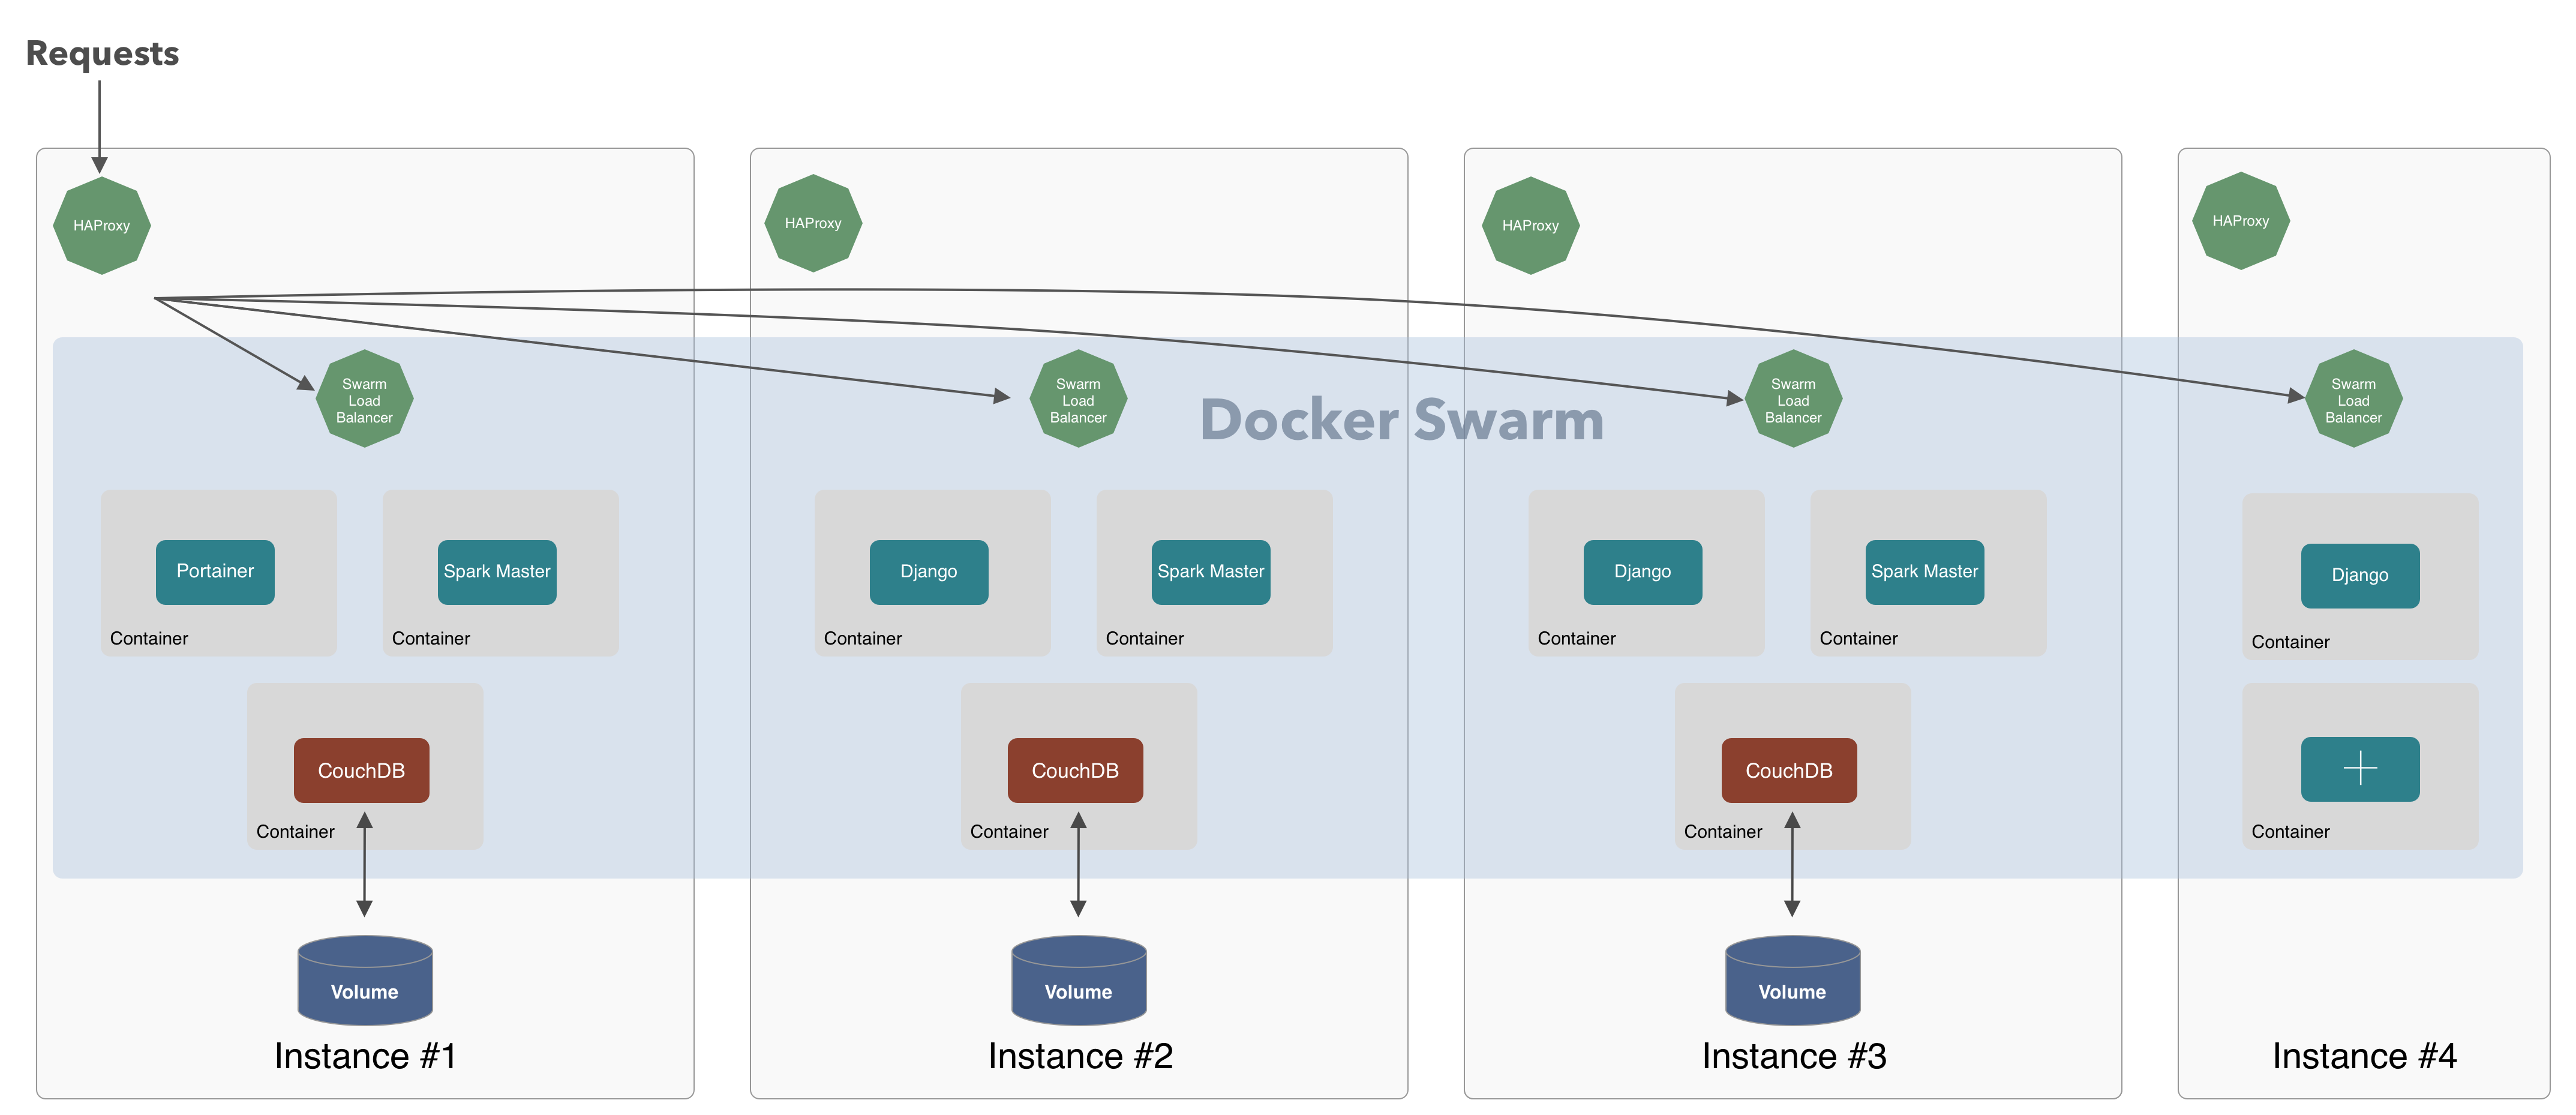
\includegraphics[width=6in]{Figures/Overview.png}
\caption{Architecture \label{Architecture}}
\end{figure*}
\begin{figure*}
\centerline{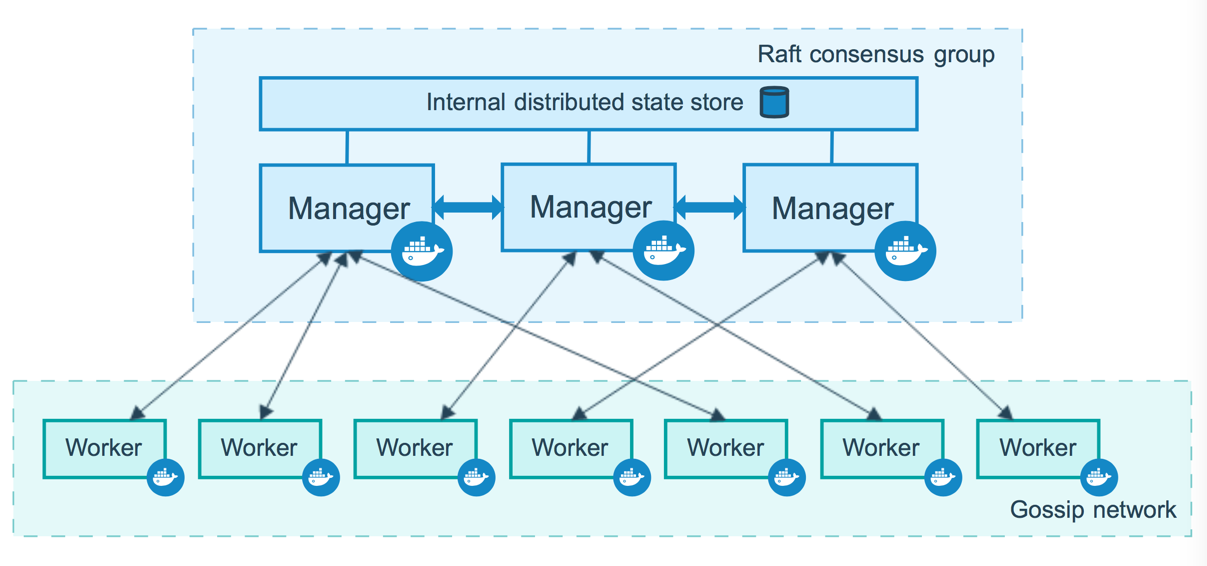
\includegraphics[width=6in]{Figures/swarm-diagram.png}}
\caption{Docker Swarm Managers \label{Docker Sarm Managers}}
\label{docker manager}
\vspace{-0.5cm}
\end{figure*}

Twitterlance is a distributed system that harvests, stores, and analyses Twitter users and their timelines. To improve the development productivity, the architecture design has been aiming at high scalability, high availability and high automation. High Scalability is supported by the combination of CouchDB, Docker, Docker Swarm, and Ansible. High availability is a design objective embedded in the error handling methods of all software components in the system, while the duplication of services also makes a contribution to this goal. The purpose of high automation is to provide a one-click solution for deployment and scaling. With Ansible and Docker Swarm, it is extremely easy to scale up the data and harvesting/analysis performance when new resources are available on the cloud. The automated deployment is designed for Melbourne Research Cloud only, where the system is currently deployed.

The system conducts two major tasks: data harvesting and data analysis. The process of harvesting consists of two phases: collecting users and collecting tweets, which can be initiated via the home page of the web application. Data analysis is implemented with the integration of Django, CouchDB, and Apache Spark, which are all running as scalable clusters.

The overall architecture is illustrated in Figure \ref{Architecture}, where HAProxy works as an external load balancer outside of the docker swarm. The Swarm load balancer works as a routing mesh that redirects requests to containers across MRC instances. Portainer is a GUI-based docker swarm controller app. Django contains a Twitter harvester and web application, in which the harvesters work in parallel. Apache Spark cluster is used for the data analysis that CouchDB does not well support. Lastly, CouchDB is configured to work as a cluster where the data storage is mounted to the MRC volumes. By default, the system requires a minimum of 3 nodes to run properly. Due to the resource limitation on MRC, Instance 4 has the least resources available, so it is created to test and showcase the scalability of the system.

\subsection{Containerisation}
\begin{figure*}
\centering
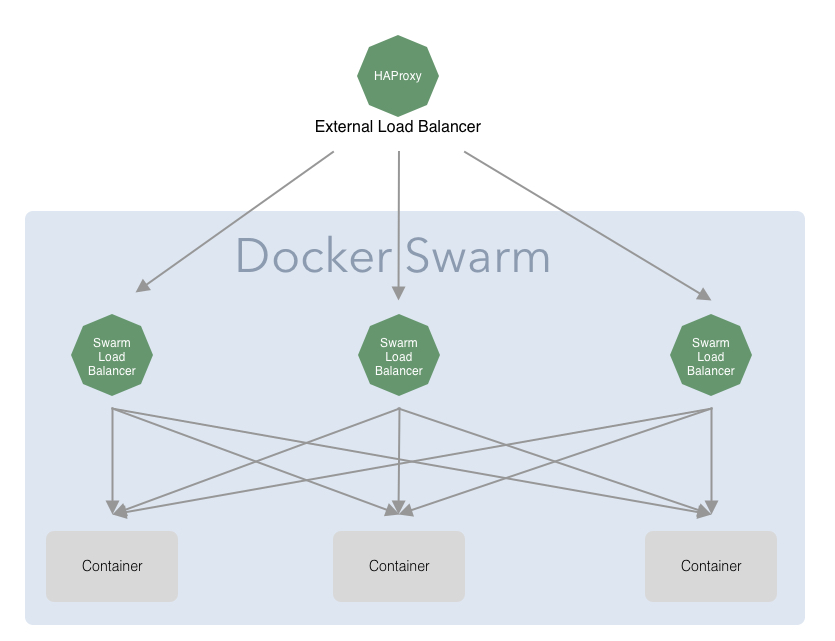
\includegraphics[width=6in]{Figures/Network.jpg}
\caption{External Load Balancer}
\label{External Load Balancer}
\vspace{-0.5cm}
\end{figure*}
Containers are a type of virtualization technologies that enable developers to encapsulate the software application along with the dependent environment. A container provides a clean environment on top of a choice of the base image. Then developers can package the application and all the dependencies in this environment into an image. This decouples the software package and the actual execution environment, which allows the package to be deployed on any platform easily. 

Instead of virtualizing the hardware, containers virtualize at the operating system level. This allows multiple containers to share the same hardware and operating system components, which is faster to initiate and consumes fewer resources than virtual machines. 

Docker is used as the containerization tool as it has the largest community with abundant open-source resources. Most of our software components are deployed within Docker containers managed as scalable services by Docker swarm orchestration tools. Docker swarm is natively supported by Docker so it does not add as much complexity as using other tools that need extra packages. Docker swarm enables a single entry point of container management across multiple host machines (either virtualized or not). It adds another layer of abstraction, in which developers do not need to be concerned about where containers are deployed. The swarm manager will assign containers in a way that all host machines are balanced on stress. It provides a simple interface for starting and stopping services without having to access all hosts. Each service is bound with a docker image and it can be set to have multiple replicas to form a cluster. Thus we were able to distribute multiple CouchDB, Apache Spark, and Django services across MRC instances and each service structured its own clusters to enable distributed storage and parallel computing. Figure \ref{docker manager} shows how swarm managers are linked to workers, where the maximum of loss is (N-1)/2 managers given N managers \cite{offical_2021}. Since MRC only allocated 4 instances to the system, it is configured to have 2 swarm managers, so that if one manager is down, the swarm can still function. 


The only component that is not a part of the Docker swarm is the external load balancer HAProxy, illustrated in Figure \ref{External Load Balancer}. Since the major entry point is one of the host IP, an external load balancer may help balance the requests to the Docker swarm. The network inside the swarm is balanced by the internal routing mesh, where all swarm nodes are balanced. This indicates that a CouchDB requests from any Django node could be sent to any CouchDB node by the routing mesh and the pressure on each CouchDB node should be balanced.

The configuration that enables CouchDB and Apache Spark to work in clusters in Docker swarm adds significant complexity to the development. The major challenge is that IP addresses are hidden and the communication endpoint is replaced by a random docker swarm task ID. Within a container, the IP addresses of other containers are not accessible. Luckily, the Docker swarm supports connection via container hostnames, which is constructed with the pattern $ServiceName.TaskSlot.TaskID$. For example, the below information printed by Docker contains the hostname of the first CouchDB node. The CouchDB nodes on other swarm nodes can access this CouchDB via \url{http://twitterlance\_couchdb.1.x072x072t8wkha8ybxp3iob4a:5984}.

\begin{center}
\begin{tabular}{ c c c }
ID & NAME &  ... \\
x072x072t8wkha8ybxp3iob4a & twitterlance\_couchdb.1 & ... \\
midibg71gftmjgb04sq747a35 & twitterlance\_couchdb.2 & ... \\
7us100fy01jyuczeovvadv4vx & twitterlance\_couchdb.3 & ... \\
\end{tabular}
\end{center}

Due to the use of proxy in containers on MRC, the hostname ``CouchDB" has to be added to the no\_proxy environment variable in Django containers so that Django can access CouchDB. By accessing the service name as hostname, swarm routing mesh will direct the requests to any node of the service.

\begin{figure*}
\centerline{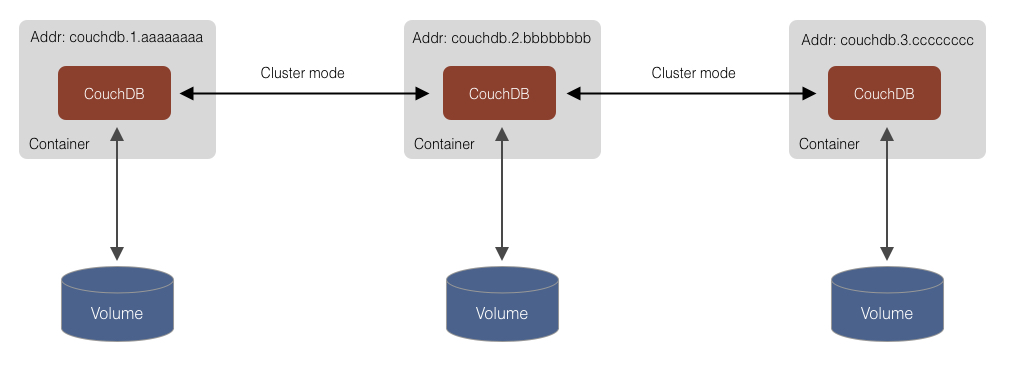
\includegraphics[width=6in]{Figures/Couchdb.jpg}}
\caption{Twitterlance CouchDB Cluster \label{Twitterlance CouchDB Cluster}}
\end{figure*}

As illustrated in Figure \ref{Twitterlance CouchDB Cluster}, CouchDB is configured to run as a cluster with multiple nodes, where the nodes are distributed on several host machines. Replicas are set to allow data recovery if any part of the infrastructure breaks down. It is set to have each node storing 2 shards, with 3 replicas per shard, which indicates that at most 2 nodes can be down temporarily. It is recommended that the number of CouchDB nodes is a multiple of 2 so that the shards can be distributed evenly.

Since each MRC instance mounts an extra volume, which is significantly larger than the default volume, it would be more flexible to place CouchDB data on this volume. The extra volume is programmatically mounted by the deployment scripts.

Docker supports three types of volumes, where one of them is placed on memory, and Volumes and Bind Mount are placed on the filesystem of the host. Although Volumes are officially recommended by Docker for many reasons, Bind Mount is chosen to be the storage method because it is more suitable for storing persisting data. Given that the data may exist outside of the container lifecycle, especially when services are restarted or redeployed, the existing data can be easily moved or ported to the new database services. An important configuration is that the path of the bind mount must exist on all swarm nodes before deploying the service. 

CouchDB cluster cannot automatically add nodes to cluster on the first-time simultaneous deployment, so Ansible will run a Python script that adds all nodes to the cluster after the first batch of CouchDB tasks are alive. Any new CouchDB node added by scaling up the service is automatically discovered by the existing CouchDB cluster. Most importantly, the configuration, including secrets and cluster settings, must be consistent on every node.  

Docker-compose is configured to assign each CouchDB container a node name with the pattern of $<Service Name>.<Task Slot>.<Task ID>$, so that the containers can communicate with each other. In a working cluster, shard files are registered to be paired with CouchDB node names in the intrinsic databases. If the Docker services are removed or restarted, the CouchDB node name will randomly change, which will cause failures in reading shards. A separate Ansible task initiated by \href{https://bitbucket.org/comp90024team39/comp90024-a2/src/master/deployment/recluster-couchdb.sh}{recluster-couchdb.sh} can be used to fix the mismatching shard-node pairs. 

The Ansible task \href{https://bitbucket.org/comp90024team39/comp90024-a2/src/master/deployment/recluster-couchdb.sh}{recluster-couchdb.sh} gathers all hosts information via \href{https://docs.ansible.com/ansible/latest/user_guide/intro_dynamic_inventory.html}{openstack\_inventory.py} and runs a Python script \href{https://bitbucket.org/comp90024team39/comp90024-a2/src/master/deployment/files/couchdb_cluster/reshard.py}{reshard.py} on every host. This enables developers to link CouchDB and shards by one script. The Python script uses a docker SDK to gather all container information on the node, and bind the local shard file names to the CouchDB service task name in the database. It needs to run on every node because the shard files are distributed across the swarm. 

\subsection{Database}

The application utilizes tweets to do different analysis scenarios, which requires the tweets to have been stored and well-prepared whenever the application needs to refer. Tweets have a standard JSON file structure proposed by the Twitter company, though the relational database is able to store the fields of that structure over different tables, a JSON file including an integral tweet can be fed to the NoSQL database. From this perspective, the application employees CouchDB, an open-source document-oriented NoSQL database, to store data.

\subsubsection{CouchDB}
The flexible document-based design enables CouchDB to store various types of data, such as AURIN data, tweets, geocodes of the cities, and Twitter API tokens. These data lead to a large volume,  and CouchDB has a promising architecture to handle big data. 
\begin{itemize}
    \item CouchDB is a distributed database, which allows users and servers to access and update the same shared data while disconnected and it can be distributed in a cluster instead of a single node to promote the performance. 
	\item CouchDB provides eventual consistency in its distributed system, which means CouchDB enables a single node to support reading and writing service and synchronizes the changes in the cluster later in incremental replication progress.
	\item CouchDB uses MapReduce methods to optimize data extraction efficiency.
\end{itemize}
CouchDB communication follows representational state transfer (REST) design, which is easy to understand and use as the zen of CouchDB relax. 

\subsubsection{MapReduce}
Reading information to satisfy users’ needs is always the core of database tasks, and MapReduce allows the database to extract data in a parallel manner. A MapReduce job consists of splitting the data into independent chunks and processing them by a map function parallelly. CouchDB provides many build-in MapReduce methods to obtain data in views, views are the group of data to meet the users’ and servers’ needs,  and this application uses \mintinline{python}{sum} function and \mintinline{python}{count} function. The \mintinline{python}{count} function counts the values of some pre-defined keys, while \mintinline{python}{sum} function counts the occurrence of an object, such as a dictionary or an array. After implementing the above two methods, the CouchDB returns the responses to the frontend ask in a shorted time, such as without MapReduce, CouchDB costs roughly 8s to return the statistical results in \mintinline{python}{users} database; otherwise, CouchDB completes the statistics task in 2s.

\subsubsection{Limitations}
In practice, though the CouchDB views use MapReduce to reduce the time consuming on grouping data, it still costs a lot of time on a large batch. For example, a view generation job on 10 GB of data will take more than 6 hours to complete at the first time, while updating the view after injection of new data also consumes a few  minutes. During the updating process, the database will compact the new data, and these two tasks make the database unavailable for users and servers to read. Meanwhile, loading all documents from a database or view in CouchDB is somewhat inefficient and inconvenient when the data volume is large. This is caused by the separations of CouchDB servers and couchjs Query servers, which brings significant overheads to the view generation and updates\cite{cd}. Furthermore, it is often inevitable for developers to update the view functions during or after collecting large datasets, in which the view regeneration will dramatically slow down the development progress. A trick can be used to speed up the development, which is separating the view that is changed often into multiple design documents, so that one updated view document does not affect other design documents.\cite{cd2}. During the development, one of our views named ``sport\_score" disappeared from the design documents due to a CouchDB issue, and it needs more than 10 hours to regenerate. We then deployed the view in a separate design document to speed up the indexing. 

Even if small new datasets are gathered progressively while the view only updates for the new data, it still causes an obvious delay in the frontend as the view is inaccessible until a batch process completes in a few seconds or minutes. 

\subsection{Web Application Backend}

All application-level programs are encapsulated in a container within the Django framework. It is the main controller of all the business logic. A typical process of using the application to collect data is:

\begin{enumerate}
  \item Launch Twitter harvesting in the front-end.
  \item Django initiates the Twitter harvester scripts.
  \item The harvester saves data to CouchDB
  \item CouchDB updates the views with the new data
\end{enumerate}

Another process that has Apache Spark involved:

\begin{enumerate}
  \item Django provides a view that calculates the fitness score of each tweet.
  \item Django submits the Apache Spark job that analyses the top 100 fitness enthusiasts in each city every hour
  \item Apache Spark cluster process the job with MapReduce and save the conclusion to CouchDB
\end{enumerate}


The process of using the application for visualizing analysis conclusion:

\begin{enumerate}
  \item The front-end requests the conclusion data from Django
  \item Django retrieves the views, transforms the data structure, and sends it to the front-end.
\end{enumerate}

Restful API is designed following its original spirits:

\begin{itemize}
\item Be able to navigate through the API without having to look at the protocol/blueprint. Each layer of the URL lists all child available resources. For example, the analyzer/ will display available children. analyzer/sports will list its children as well. The resource that does not have a child will return to the resource state.
\item The Restful resources are all nouns, which indicates that the user should always firstly get, and then modify, followed by a post for update.
\item PUT method is used to create a resource, while POST is used to modify.
\end{itemize}

All restful API are listed in the appendix.

MRC proxy needs to be configured correctly in Django containers so that it can access Twitter. A subtle caution is that hostname ``CouchDB" needs to be added to the ``no\_proxy" environment variable so that Django can access CouchDB via \url{http://couchdb:5984/}, which cannot be recognized at the proxy.   

CouchDB Python packages are redundant as CouchDB itself supports restful API. 

\begin{figure*}
\centerline{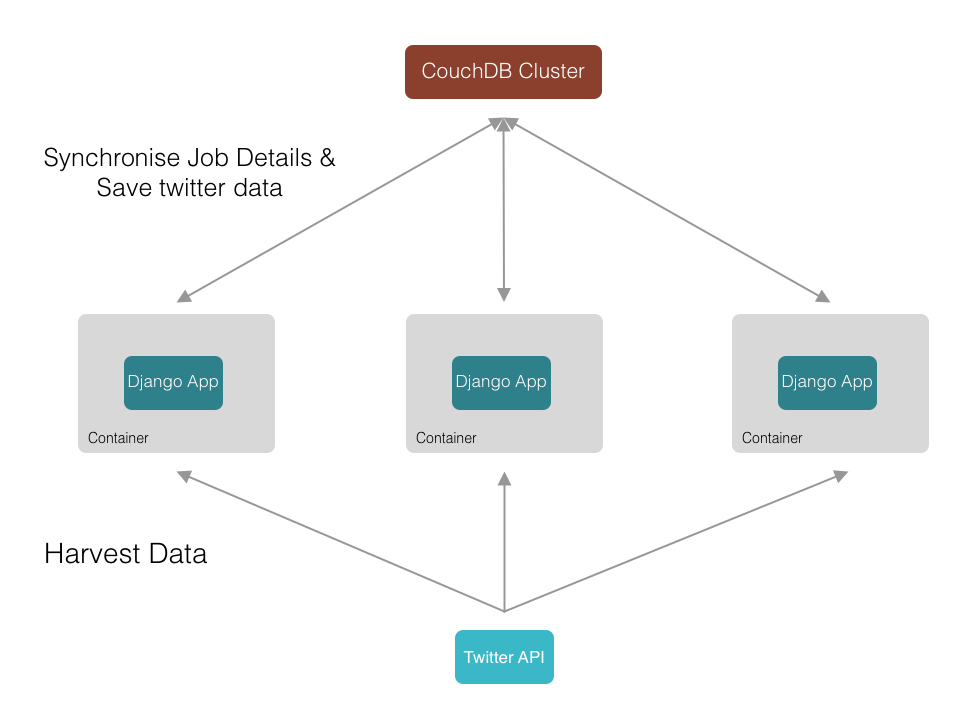
\includegraphics[width=6in]{Figures/Django.jpg}}
\caption{Twitterlance Django Cluster \label{Twitterlance Django Cluster}}
\end{figure*}
\begin{figure*}
\centerline{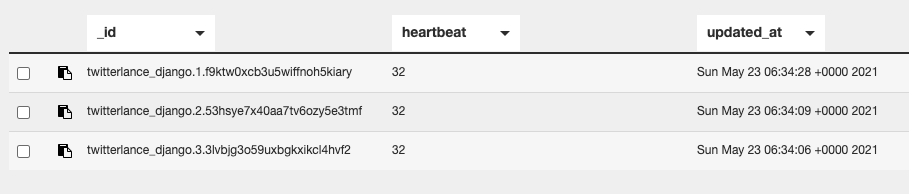
\includegraphics[width=6in]{Figures/heartbeat.png}}
\caption{Django Heartbeat \label{Django Node Heartbeat}}
\end{figure*}

Large-scale Twitter harvesting is extremely time-consuming, where they wait on network response and the Rate limit from Twitter occupies most of the time. In a parallel harvester, the number of nodes and API tokens is the most important factor rather than computation power, as it does not require much computing. Therefore, the system is designed to contain multiple harvesters within the Django framework, which provides the interface to job control. 

The Twitter harvester can be started and stopped by the job control panel in the front end. Jobs are scheduled every minute or hour by cron. Each job will check its status in Jobs database every minute. If it is on a "ready" status, it will start running the Python job and update the status to running. For the parallel tweet search job, every node registers itself in the job document, and the last starting node updates the status to "running". 

The Django cluster model follows the same paradigm as MPI, where the message passing is handled by CouchDB. \ref{Twitterlance Django Cluster} shows that each Django node registers its node name in CouchDB ``nodes" database by a minutely scheduled heartbeat cron job as shown in Figure \ref{Django Node Heartbeat}. One of the difficulties is to remove the disconnected nodes once the service is scaled or re-deployed. In attempting to use the container hostname for connection tests, an issue is that the MRC proxy cannot resolve the hostname. Furthermore, the specific hostnames in the pattern of $ServiceName.TaskSlot.TaskID$ cannot be added to the no\_proxy list due to random $Task ID$ generated at swarm task deployment. Since Django node cannot directly access each other, an algorithm was implemented to periodically compare the heartbeat ``updated\_at" field with the current time, and if a node has not been submitted a heartbeat for over 5 minutes, it will be recognized as disconnected and will be removed from the database. 

When parallel harvesters start, each node will be able to find its own assigned portion by calculating the position of its rank in the total number of nodes. The aggregation of tweets or user data is simply completed by a CouchDB PUT method. Since the only shared information is the total number of nodes and it is only accessed once, the network performance of CouchDB would be sufficient for this task. This does not require MPI or other distributed models and tools so the system complexity remains. 


\subsection{Web Application Frontend}

\subsubsection{Framework}
The front-end includes a homepage, a map page, a statistics page, and some buttons for doing backend control. Figure \ref{frontends} is the structure of our front-end. We managed the main structure of our front-end with Bootstrap, one of the most popular HTML, CSS, and JS library. Most details of our front-end are amended by CSS, for example, the font family, font size, shadows of boxes, and so on. All the static resources were load from the Django backend. Charts in the frontend were plotted with the Char.js library and ECharts library \cite{LI2018136}. The Django backend provided the resource to the frontend with RESTful URL, then the front-end was connected to the backend by jQuery. jQuery is a JavaScript library that simplifies the programming of sending ajax requests to the backend. The following is an overview of the architecture of the front-end system. Data analysis results and the job status will be displayed in the front-end, and we can start the twitter harvest Job by clicking the button in the front-end. 
\begin{figure*}
\centerline{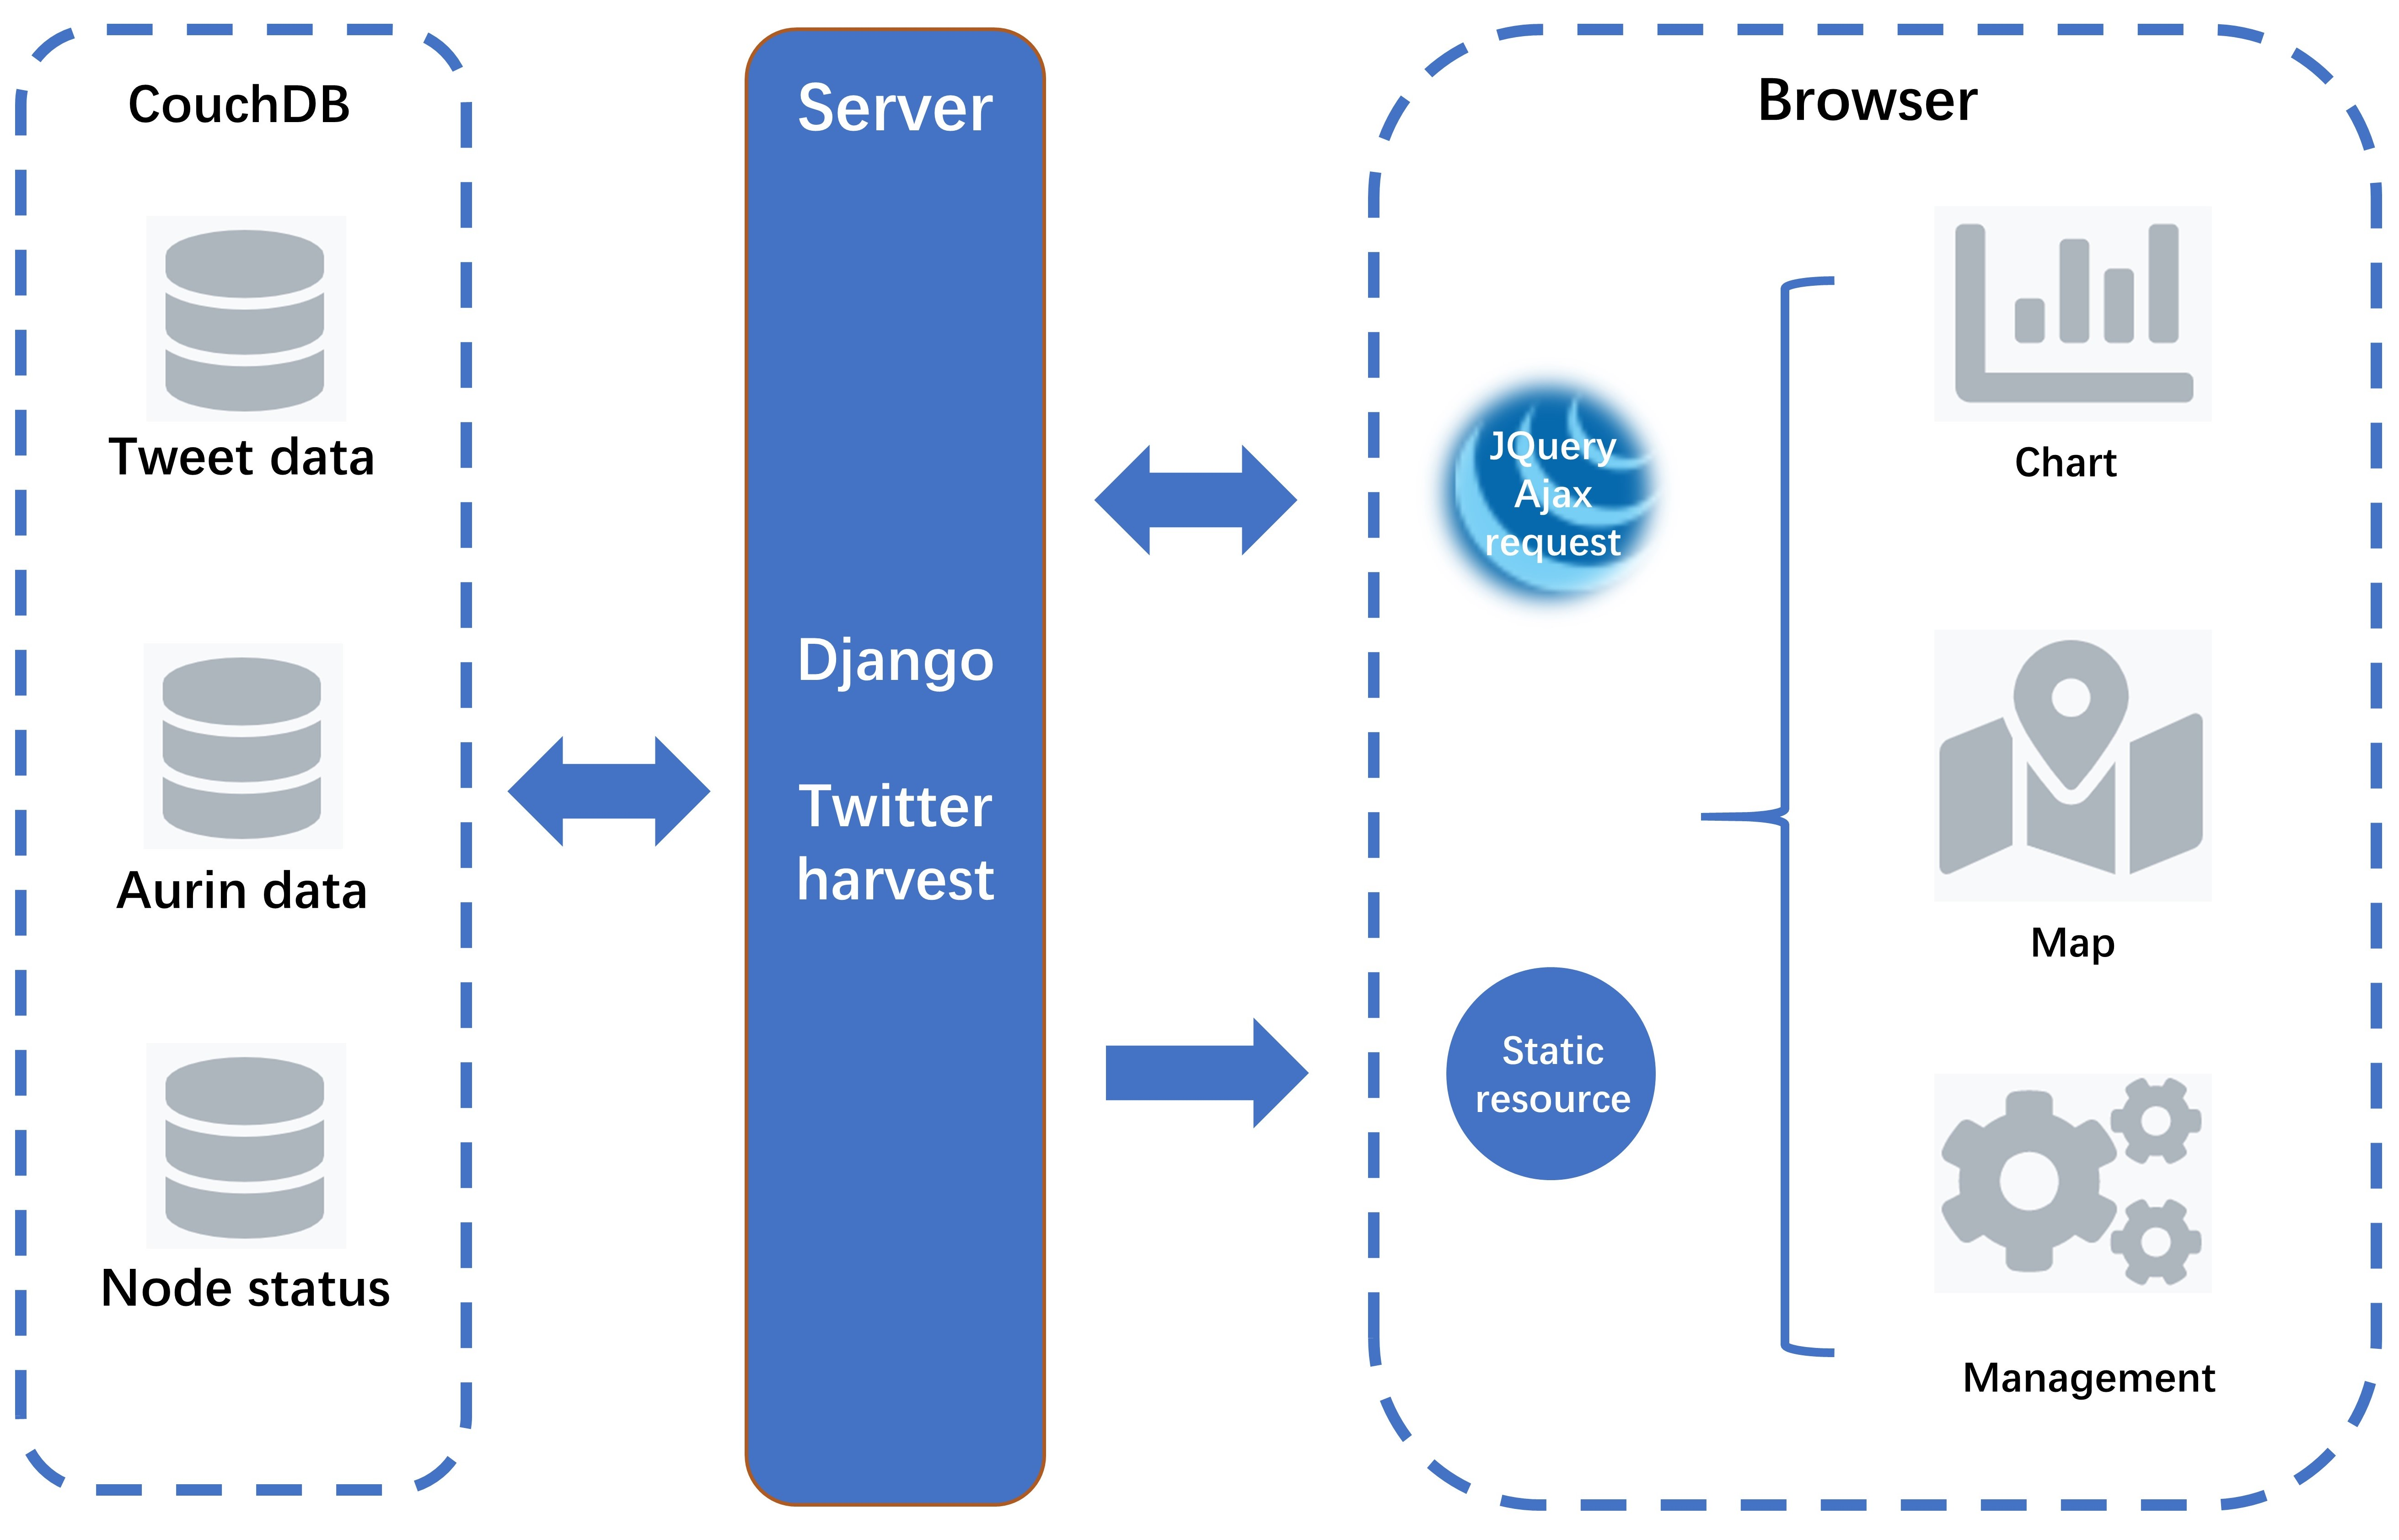
\includegraphics[width=6in]{Figures/FrontendStructure.JPG}}
\caption{Front-end Structure\label{frontends}}
\end{figure*}

More to mentions, during the view regeneration on new data intake, typically when Twitter stream mode is turned on, the frontend will request the view in a loop of retries, so that the data will be available as soon as the view finishes processing the new data. 

\subsubsection{Map}
The map page shows the pattern of sports tweets in each city and is created by using JavaScript, CSS, and HTML. While the base map layer is made through Mapbox, which can be accessed through style URL and access token. In general, there are six points representing six cities, namely, Melbourne, Sydney, Adelaide, Brisbane, Perth, and Canberra, whose size depends on the number of tweets. When the user hovers the mouse over any of the points, a pop-up containing descriptive statics, a real-time interactive bar chart, and a line graph appears, which are made by using Apache ECharts. We also included pop-up effects in those two figures just in case the user would be interested to see the exact number. Except for showing the cities’ information, we add a geocoding control by using Mapbox geocoding API, enabling users to search a place on the map.

\subsubsection{Statistics}
On the statistics page, information from Aurin and Twitter data were shown. At the top of the webpage, three dashboards that include the total number of users, the total number of tweets, and the amount of sport-related tweets were placed. Below the dashboard, there are several charts. The charts show the data extracted from Aurin (median age, gender ratio, education index, unemployment rate, and income) and the analyzed data which are the three scenarios. Three scenarios are the most vibrant city (the city with the highest sport score), popular sports, and fitness enthusiasts. All the charts were made by Chart.Js package and data were getting from CouchDB by using jQuery which details will be explained in the Data Analysis section.

\subsubsection{Limitation}
The front-end code contains repetition and hard-coded patterns that can be further engineered. For example, The city names could be encapsulated so that the expanded city list is reflected in the front end automatically. 

\subsubsection{Deployment}

The production deployment and scaling have been recorded as a video on \href{https://youtu.be/cqmxZdLdOyk}{Youtube}.

The entire system is designed to be running on Melbourne Research Cloud. Ansible scripts are developed to create security groups, volumes, and instances on the cloud via the OpenStack module. We provided a one-click solution that allows the developer to deploy or scale up the entire system with one click. This section explains the deployment methods. Refer to the appendix for the deployment user guide. Each folder in the project repository contains a readme file that describes the configuration details and code components.

Ansible is chosen as the main deployment tool because it has a large community base, where numerous modules are available to the automation. The deployment is completed in 2 phases: infrastructure and application. Infrastructure includes the creation of security groups, volumes, and instances on Melbourne Research Cloud (MRC). Authentication is ensured by using SSH and MRC master password. The team shares a single project on MRC, where all software components are deployed.

Some nodes in Docker Swarm are marked as $``couchdb=true"$ and $``spark\_master=true"$, which means only the marked instances can deploy CouchDB and spark master. These marks can be changed on Portainer (accessible from the ``Manage" button on the web app) if CouchDB needs to be scaled up. 

One of the main challenges of deployment automation is to obtain the instances' details after they are created. After researching the OpenStack project, we found a convenient Python script \href{https://docs.ansible.com/ansible/latest/user_guide/intro_dynamic_inventory.html}{[openstack\_inventory.py]}, which automatically loads the hosts' information into Ansible, so that the deployment starts from allocating resources on MRC and ends when all applications are configured without asking the developer to find and enter any information manually.

The application deployment process starts with the configuration of the environment, including directories creation, file permission setup, package installation, Docker swarm setup, and then followed by Docker stack deployment and application initialization. Docker Swarm initialization is the most difficult part to develop among the aforementioned steps. It requires one host machine to initialize the Docker swarm, which generates a token for joining the swarm. The initial host needs to find its IP address that is accessible from other hosts. When the join token and IP address are available, all other hosts should run the Docker swarm join command followed by the token and IP address to join the swarm. It is important to ensure that the security groups are correctly set so that all necessary ports are open for Docker swarm, CouchDB, and Django clusters. 

Another challenge is to share the token and swarm the initial host IP address across all Ansible hosts. Initializing swarm and joining swarm are separated as two plays so that the token and IP are saved in a dummy host variable shared across plays before other hosts join the swarm. All the details of the host machines (MRC instances) can be found in the Ansible inventory provided by \href{https://docs.ansible.com/ansible/latest/user_guide/intro_dynamic_inventory.html}{[openstack\_inventory.py]} script.

CouchDB cluster needs an extra script to initialize during the first-time deployment. When CouchDB nodes are ready, Ansible will invoke a Python program that adds all the nodes to the cluster. Environment variables and CouchDB initial configuration need to be set carefully so that the CouchDB nodes can run in the same cluster.

When the deployment is completed, it is recommended to quickly scan the files and verify if all the files, mounts, and directories are in place so that the risk of deployment fault is minimized.

\subsubsection{Partition}

Partitioning is a part of database management where a large table is splitting into multiple small tables, whose main purpose of partition is to speed query. For CouchDB, one of the limitations is that no more than 10 GB of data can be stored in each partition (recommended by the CouchDB developer). To apply partition, as well as query faster and efficiently, once tweets are stored in the database, they are partitioned according to their location by setting each entry’s ID as “{city}: ID”. Therefore, tweets posted in the same city have the same partition key (second indices).  When checking the view result of any city, we can just simply add a city name after “\_partition”. For example, by using $/tweets/\_partition/Melbourne/\_design/sports/\_view\\/total$, we can get the total number of sports tweets in Melbourne. 

We had planned to partition the database by cities, but only realised the 10G size limitation when most data is in place. The solution is to remove the partitions, as either user or city data could potentially grow over 10 GB. The shard reading speed optimisation by partitioning is not a priority as the bottleneck is at the view query  communication with couchjs server. It is estimated to take 2 days to migrate the partition method and the relevant code, which is not a difficult job but CouchDB will consume 10-15 hours to rebuild the views. Due to the limited time-frame, we have left it as is. If the user continues to harvest a very large amount of data, it may potentially hit the size limit.

\subsection{Scalability and Automation}

Scalability and automation are the most important design objectives in Twitterlance to minimises the future deployment and extension work while data grows. Although it is a non-trivial job to develop such a system, they will save a tremendous amount of time for future scaling-up tasks and extensions. In the scope of  Twitterlance, every functionality is encapsulated into a single click solution, such as deployment, start and stop harvesting, and data analysis. Robustness has been maintained at an acceptable level, as it will not break unless under stressful usage. 

The scaling of MRC instances is supported in a separate Ansible script, where new volumes and instances are created. The developer only needs to change a few lines of settings in the Ansible script to specify the new resources. When the MRC instances are ready to run programs, the developer can scale up and down the Docker services in Portainer, which is a tool that we use to manage the swarm. The “Manage” link on the web application is linked to Portainer, where the default username and password are “admin” and “password”. Scaling up Docker services such as harvesters, Apache Spark workers, or CouchDB nodes is as easy as turning on a television in Portainer. The services are set to automatically connect to their clusters.

The user or developer may scale down the computation clusters: Apache Spark or Django, but it will not be meaningful because computation demand will always grow as data grows. It is complicated and not recommended to scale down any CouchDB nodes because CouchDB data is bound with the file system on the host instance on MRC. The removal of CouchDB nodes requires developers to manually merge shard files, which is a complex and risky job for production. Moreover, it is unlikely that we remove any data as the cost of data storage is trivial compared to other services. However, there may be requirements to move CouchDB nodes to other host instances.

\subsection{MRC}
The Melbourne Research Cloud is Infrastructure-as-a-Service. It provides users with virtual computers, networks, and disks. Users can deploy and run any software, including applications and operating systems on MRC. Users can also choose the version of the operating system, data storage method, application deployment type without contacting any manager. At the same time, users do not need to manage any IT equipment or data center facilities. Most importantly, it is completely free of costs for us. 

MRC is extremely helpful for researchers, for it can provide researchers with a huge amount of processors, lots of memory, and a great number of computers. The virtualization technology of MRC includes application virtualization and resource virtualization, which breaks the boundaries of time and space. Further, MRC supports multiple languages, which is friendly for foreign researchers.

All the services of Twitterlance are deployed on Melbourne Research Cloud. Overall, the MRC instance creation can be fully automated using Ansible and OpenStack SDK. MRC image creation is unused as Docker containers do not depend on environments. A fresh deployment always starts from an empty project on MRC. However, scaling up is not as easy as the first-time deployment, because the developers need to specify the names of new instances to be created by the Ansible Task. It will be more convenient if the deployment tools are further encapsulated so the developer only needs to enter the scale when scaling up. 

In attempting Ansible development, MRC instances were frequently deleted and re-creating for testing purposes. An issue occurred where volumes could not be deleted due to the mount to deleted instances, which was resolved manually by technical support. It is inevitable that a complex cloud platform such as MRC runs into a problem due to stress, system weaknesses, or abnormal usage. 

MRC instances can be accessed via SSH and VPN, which ensured security but VPN brings inconvenience and inaccessibility. 


\subsection{Data Sourcing}
\subsubsection{AURIN}
Six cities are explored and analysed in this research, and the cities’ boundaries are defined by the greater capital city statistical area (GCCSA). The datasets chosen from the AURIN platform are JSON files between 2016 and 2019. After pre-processing, cities’ profiles are created and combined, including facts such as income, education, housing price, demographic information, and unemployment rate, etc.

\subsubsection{Sport List and Challenge Rank}
The sports list includes 76 sport types and their challenge ranks. ESPN published 60 sports rankings according to the degree of difficulties, where boxing is proved to be the most demanding sport and fishing is the least. We pre-processed the list by adding 16 extra common sports in Australia into the list manually, such as “footy”, “AFL”, “F1”, “hike”,” jog”, etc. While those newly added sports are scored according to their similar sport types which are already on the list

\subsubsection{Twitter Harvesting}

The Twitter harvest utilizes Twitter API to get tweets from Twitter. Due to the limitations of the Twitter API, ordinary users cannot get search results for specific words before 7 days, but there is no time limit for crawling the user's timeline. This system bypasses the time limit of Twitter by first finding users and then crawling the timeline, thereby obtaining a relatively complete database. This harvesting system consists of searching, updating, and streaming, the first two parts employ search API, and the last uses stream API.

\paragraph{Components}
The search part tends to find the brand new users from the tweets, and to ensure the users are brand new, the search gets the full user list via \mintinline{html}{GET /users/_all_docs} and checks the returned users from the Twitter query.  The query only contains a whitespace ‘ ’, since almost all the tweets in English use whitespace to separate words, the search can obtain as many brand new users as possible. The update part aims to crawl the timelines for the brand new users and update the timelines for the users with an outdated update timestamp. However, some Twitter fanatics and official accounts post too many tweets, which is irrelevant to our scenario, the system only obtains the first 3,000 tweets for one user. The stream listens to the tweets in real-time. Because monitoring efficiency of the stream is not high and the amount and flow of data are small, once a new user is discovered, they and their timeline can be directly added to the database without worrying about the overloading of \mintinline{html}{POST} requests.

\paragraph{Data Structure}

Twitter proposed snowflake algorithms to ensure it can generate a unique user ID and tweets ID \cite{10.5555/110778.110783} \cite{10.5555/70413.70419}, thus the CouchDB can set the user/tweet id as the id to avoid duplication issues. However, the tweets database has a large volume, which needs a partition to improve its performance. Since the application aims to investigate the sport situation over cities, using the city name as the partition primary key is nature. Though implementation of partition improves the query efficiency, the partition database in CouchDB does not support the custom MapReduce method, which limits the scope of views.
The user fields consist of id, city, and update timestamp, the id is the user id, the city is where the user has been found, such as Melbourne, Sydney, and Perth, and the update timestamp records the timestamp that the application updates their timeline. The timestamp format follows Twitter style.
The tweet fields are id, city, user id, and value. Due to partition, the id consists of city, colon, and tweet id, which provides a unique id for each tweet. And value is the whole tweet object.


\paragraph{Algorithms}\footnote{All the details of algorithms are shown in the Appendix pseudo code part.}

The search algorithm consists of \mintinline{python}{search_user} function and \mintinline{python}{run_search} function, and this algorithm tends to find a fixed number of brand new users, this number comes from front-end inputted by the application user. Brand new users are the users out of the \mintinline{python}{users} database. Running this algorithm in a parallel manner cannot guarantee the system will add to the number of Twitter users the application user wants to add. Because some instances may wake up later than others, and it obtains the  \mintinline{python}{users} database that other instances have added some brand new users in. Completing the search job on one node can solve this problem. Meanwhile, assigning search user jobs across nodes evenly does not save much time. Therefore, the system only employs one node to complete the search user job.

As for error handling in search users, the key idea is moving to the next token while a fatal error occurs. Once a fatal error occurs, the search user function will return the \mintinline{python}{maxid} of the current batch of tweets and the number of how many users have been added, then the algorithm will move to the next token and commence a new search user function at that breakpoint. Though our group only has a few tokens, we can build a token pool by expanding the token list 10 times and randomly shuffling the token pool. Expanding allows the system to try enough times, and random shuffling enables different instances to use distinct tokens to avoid rate limits in Twitter API. Meanwhile, each user has a token pool, that is the token pool is the innermost loop. In sum, this design assumes that tokens will not be consumed easily, trying different tokens can solve both the short-term network connection problem and the exhaustion of a certain token. As for CouchDB, the \mintinline{python}{PUT} request deserves the most attention, that is feeding the user data to CouchDB. For each \mintinline{python}{PUT}, the algorithm will try 5 times maximally and each retry will sleep 10s, if the CouchDB returns a good status code, such as 200, 201, and 202, the algorithm will start the next search to harvest new tweets; otherwise, it will continue work on the current batch tweets. This design makes full use of the Twitter query results and allows short-time connection error with CouchDB. 

The update algorithm also consists of \mintinline{python}{search_tweets} function and \mintinline{python}{run_update} function, which aims to update the user timeline without an update timestamp or with an outdated update timestamp, the former allows to search 3,000 tweets maximally and the last limitations range from 400 tweets to 3,00 tweets. Unlike search user algorithm, update algorithm works in a parallel manner, since each city has almost 10,000 users and the searching timeline for one user is independent with others, parallel processing can greatly improve efficiency. The algorithm automatically assigns tasks to each instance evenly. For example, there are 3 nodes and 10 users in CouchDB, the algorithm will assign an index to each node, such as 0, 1, and 2, and it evenly splits the 10 users into 3 intervals and assigns them to the node respectively, [0, 2] for index 0 nodes, [3, 5] for index 1 node, and [6, 9] for index 2 node, then executing the \mintinline{python}{search_tweets} function in each instance. The assigned rule follows left close, right open, thus, each node will be assigned to the same volume task. \mintinline{python}{GET \{db\}/_all_docs} in CouchDB returns the id of all documents in an ascending manner, which promises the user list in each instance has no intersection.

The update and search share the same idea to handle the fatal errors, but the update doesn't allow breakpoint retransmission. In update progress, the function will \mintinline{python}{PUT} the user and their timeline into CouchDB, and it is difficult to tell which progress failed and retry at the failure point. To simplify the code and logic, the algorithm only allows the two \mintinline{python}{PUT} progress to success at once.

Comparing to the update and search algorithm, the logic of the stream algorithm is more simple and straightforward. Similar to search and update algorithms the stream algorithm consists of \mintinline{python}{run_stream} function and \mintinline{python}{stream_tweets} function. The stream algorithm is aimed to listen to the instant (several hours ago) tweets in target areas. In-stream progress, the function will firstly identify which city the tweets come from. Then, check whether the user is in our CouchDB. If the user is in our CouchDB then store the single tweet into the CouchDB(stream API can only get instant tweet). If the user is not in our CouchDB then store the user and his timeline into CouchDB and add a timestamp to the user. The timestamp will be used by \mintinline{python}{stream_tweets} algorithm. Stream algorithm works in a single node. In the experiment, we found that when listening to the single city the tweets harvest speed is extremely slow, nearly 2 tweets per minute. When expand the listen to the area of four cities, the stream algorithm will get about 6 to 8 tweets per minute. working in a parallel manner will not increase the work efficiency of the stream algorithm in our condition.

For error handling in stream, during the development stage, we only found network connection errors. Handling this error is relatively simple. When a network connection error takes place the algorithm will sleep for few minutes, and continue the job after sleep. When the connection was stable, the stream will listen to the instant tweets again. 

\paragraph{API keys and Limitations}

Both search and stream API were accessed via tokens which were generated by using the Twitter Developer account. The accounts used in this project are all standard accounts, so the tokens generated by these accounts have some limitations which are mainly related to search API. The limitations are that we can only search the tweets within 7 days and the maximum number of tweets we can get from each user's timeline is 3500. Moreover, the search API only accepts 180 requests per 15 minutes. As a result, when doing Twitter harvesting, the number of search tweets was limited, and the speed was slow. Another problem related to tokens was met apart from those limitations: tokens were suspended several times due to the spam groups of Twitter. Token disable is a huge issue when doing Twitter harvesting. To avoid that, all tokens were stored in the token database, so that we can replace or remove the disabled tokens easily from the database. This allows API to be accessed via the working tokens only.

\begin{figure*}
\centerline{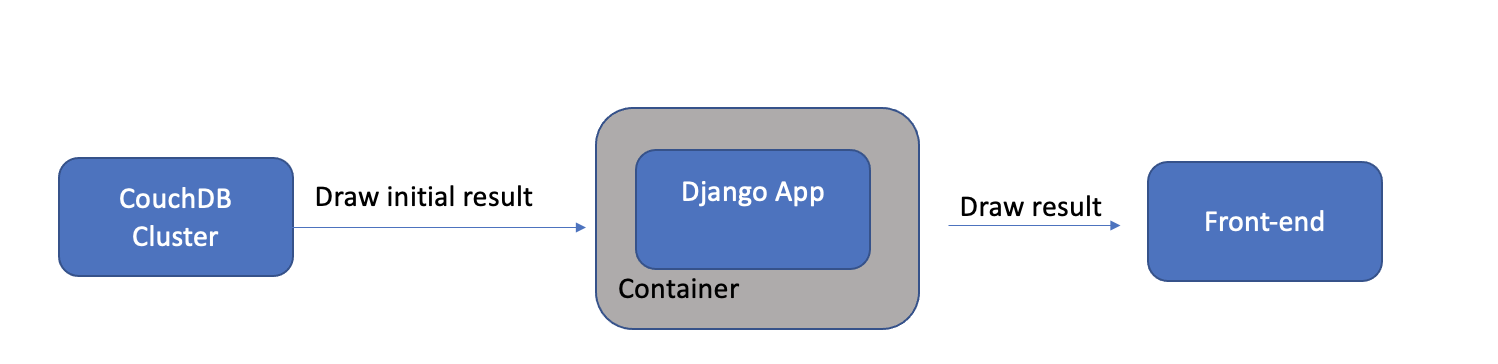
\includegraphics[width=6in]{Figures/couchdb-django.png}}
\caption{Map Reduce in CouchDB \label{couchdb and django}}
\end{figure*}
\paragraph{Implementation and Limitations}

In MRC, the search script costs 10s $\sim$ 15s to find a brand new user in one city, and the update script harvests the timeline for one user in 5s, and these scripts have run 13 hours in MRC without throwing an error. Thus, the Twitter harvest has a promising performance. 

There are several limitations posed in the Twitter harvest system:\\
\begin{enumerate}
    \item Though the system can handle the breakpoint while running the script and cancel these tasks in the frontend via job control bottoms, the user can not pause and resume the search, update, stream progress.
    \item The algorithm can not handle long-time connection error. 
    \item The system fails to obtain the timelines of some users due to authorization issues, this unauthorized means the user sets their account as private status, which does not allow the public to access their tweets. Due to the timeframe, the system fails to handle this situation.
    \item It’s quite inconvenient to check the logs overall. The Portainer provides an incomplete overall log with a wrong timestamp, which halts the checking progress.
    \item Tokens are always inadequate. Applying for a Twitter development account is difficult, and Twitter does not provide a clear measurement about the usage, thus we don't know when the token will run out of its usage. 
    \item Twitter development accounts are not in a stable status. Our group has crawled data in a gentle way, but two accounts have been suspended several times.
\end{enumerate}



\section{Data Analysis}

There are three scenarios included in our research, namely, the most vibrant city, the popular sports and fitness enthusiasts. 

Data utilized here are from Twitter, AURIN, and ESPN, which are stored in CouchDB. Twitter users typically post varieties of content, where texts, locations, and usernames are used here to identify patterns in three scenarios. As for data from the AURIN platform, we assume these are relevant in the context of the vibrant city (scenario 1). To recognize the fitness enthusiast (scenario 3), the tough sports ranking from ESPN is one of the key measurements.


\subsection{Scenario analysis}

\subsubsection{Overview}
AURIN data can be easily stored in CouchDB and imported after selecting features and merging results through Python. As for the sports list and difficulty ranking, we add different tense of each sport as well as its synonymous manually before they are stored in two lists or arrays in views. While for original Twitter data on CouchDB, Django application, CouchDB map reduce and Spark are utilized to obtain the result. 

For Twitter data, the CouchDB view is defined firstly to extract special data, which includes a map function written in JavaScript and a reduced function embedded in the database. Django then sends a \mintinline{python}{GET} request to draw results from the CouchDB view through CouchDB REST API. After feeding the initial result to Django, it then invokes the analyzer Python code to further process the data. Finally, the conclusion is constructed through the Django view, which can be accessed from the Django REST framework, and then can be loads to the maps, graphs, and charts, and this is illustrated in Figure \ref{couchdb and django}.

An emerging challenge during the analysis stage is that only predefined reduce functions are supported by CouchDB, such as \mintinline{python}{_count}, \mintinline{python}{_sum}, etc, which might be hard for us to gather the result for scenario 3 analysis. To address this issue, Spark application is introduced, whose details is described in scenario 3. 


\subsubsection{Scenario 1: The most vibrant city}
Key characters of being vibrant are assumed to be energetic, enthusiastic, active, healthy, and alive. Therefore, seven elements are considered when we spot the most vibrant city, including factors generated from AURIN, such as gender, median age, median income, unemployment rate, and education levels, as well as the measurements generated from Twitter (the number of sports tweets). The score of each factor is given to every six cities from 1 to 6. For example, the more unbalanced the gender distribution in a city, the more points the city will lose. If the city's educated rate ranks the least, then this city will gain 1 point in terms of this factor. While in the city's rank the highest in educated rate, 6 points will be earned by this city. 

\paragraph{CouchDB MapReduce and Django view}

One of the key measurements of a vibrant city is the number of sports tweets post by the users living in this area. Assuming the more they post sports tweets, the more they enjoy workouts and are active. To obtain the total number of sports tweets in each city, MapReduce in CouchDB is used to filter and summarize tweets including any 1 of 75 sport types by using the reduce function \mintinline{python}{_sum}. Specifically, in the map function, we use 75 emit(key, value) functions where the key is tweet ID, and the value is a set including 75 sports with one of the sport's values being 1. If the current tweet text contains any sport, an entry then is created in the view result with the value of the sport equals 1 in the value section. By using \mintinline{python}{_sum}, it sums up values of all entries according to sport type. After that, the Django view is used, to sum up, all the sports results for each city by replacing the city name (partition name) in CouchDB restful API. 

\begin{lstlisting}[language=JavaScript, caption= Map Functions for Sports Tweets, backgroundcolor = \color{white}]
function (doc) {
    var sport = /[^a-zA-Z]racing[^a-zA-Z]/;
    if (sport.test(doc.val.text.toLowerCase())){
    emit(doc._id, {`racing': 1, `gokart': 0 ,...,`diving': 0}); //75 sports elements
    
    var sport = /[^a-zA-Z]gokart[^a-zA-Z]/;
    if (sport.test(doc.val.text.toLowerCase())){
    emit(doc._id, {`racing': 0, `gokart': 1, ,...,`diving': 0});
    
    ... //the rest emit functions 
    
    var sport = /[^a-zA-Z]diving[^a-zA-Z]/;
    if (sport.test(doc.val.text.toLowerCase())){
    emit(doc._id, {`racing': 0, `gokart': 1, ...,`diving': 1});}
\end{lstlisting}

To analyze the sports trend of each city further, the number of sports tweets of each city from 2019 to 2021 is gathered. Specifically, 3 views filtering sports tweets in 2019, 2020, and 2021 should be created respectively in CouchDB first, with the reduced function \mintinline{python}{_sum}. The map function is very similar to the one mentioned above, both of them filtered sports tweets, while this map function adds one more condition. The method \mintinline{python}{date.getFullyear()} is used here to filter related yearly sports tweets. After the view result is initialized, we use Django view to invoke the analyzer code and call the restful URL, which loops 3 years for each city. Finally, the result is returned through web browsable API on the REST framework. 



\paragraph{Result}

\begin{figure}[H]
\centerline{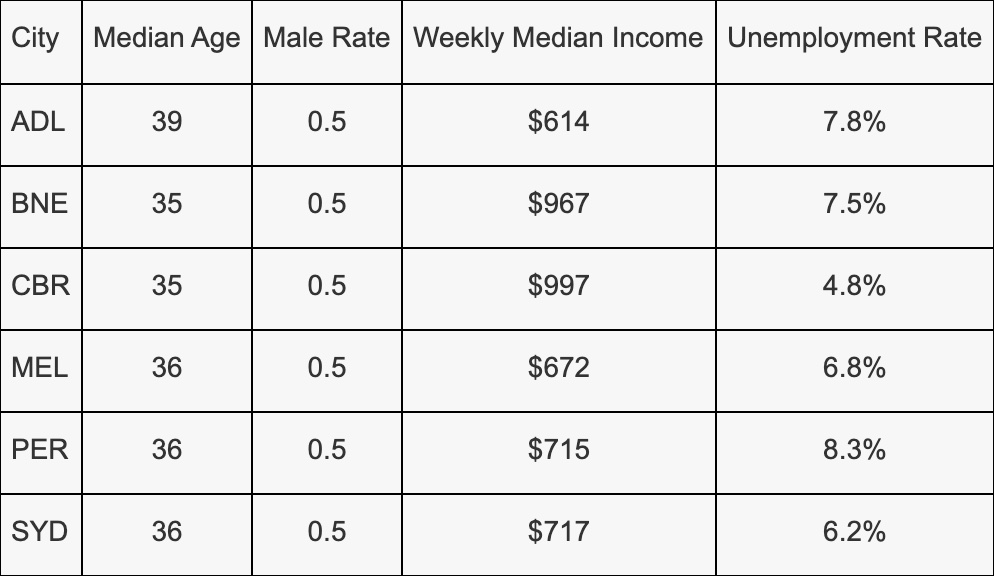
\includegraphics[width=3in]{Figures/age,income,gender.jpg}}
\caption{Age,Income, Gender and Unemployment\label{Age,Income, Gender and Unemployment}}
\end{figure}


Females and males are evenly distributed across four cities, while the median age shows a different pattern. Adelaide had the oldest median age of six capital cities at 39 years, followed by Melbourne, Sydney, and Perth at 36, while Canberra and Brisbane were the youngest, at 35. Interestingly, it is also people living in Canberra have the highest median income, nearing \$1000 per week, while the median income in every other state city ranges from \$600 to \$700 (Figure \ref{Age,Income, Gender and Unemployment}). As for employment and education, the unemployment rates across six cities are all under 9\%, with the highest number seen in Perth and Adelaide, and the lowest in Canberra, at around 5\%. Interestingly, Canberra is ranked the most educated capital city based on percentage, as well as has the highest number of people with a bachelor’s degree or higher. It is Adelaide, however, ranked least with an educated rate (Figure \ref{education}). 

\begin{figure}[H]
\centerline{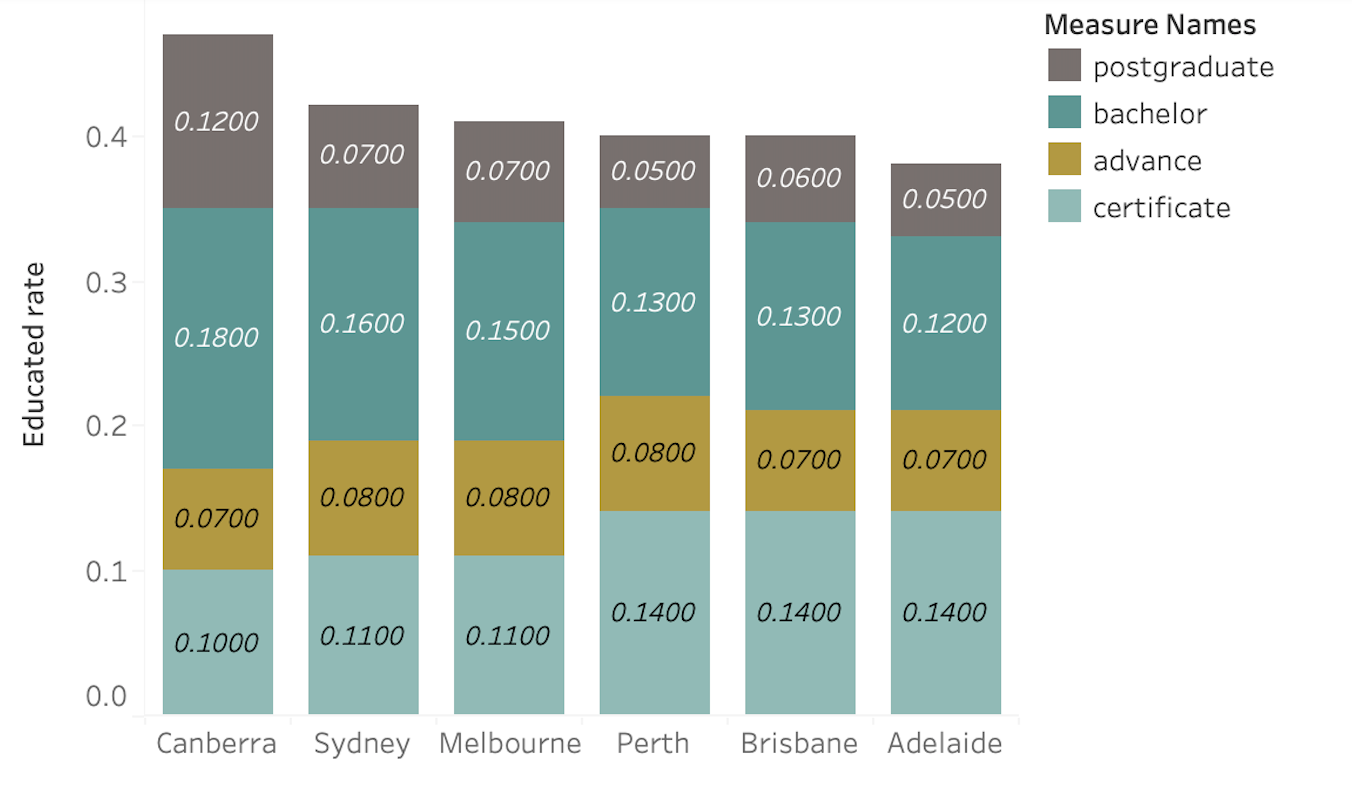
\includegraphics[width=4in]{Figures/education.png}}
\caption{Education Levels\label{education}}
\end{figure}

Regarding the sports tweets, this result is shown on the map where six circles represents for six cities and the circle size depends the number of sports tweets posted in the city (Figure \ref{map}). Adelaide posts the most sports tweets, which is followed by Melbourne and Sydney, while Perth and Brisbane post the least sports contents. By taking account of the number tweets of each area, the sports tweets ratio is used as a more objective measurement here (Figure \ref{fig:sports ratio}). Users in Adelaide still dominates in posting the sports-related content, at 2\%, which is more than twice as high as the percentage in Melbourne. It is worth pointing out that sports tweet content percent in Perth ranks the second, while users in Sydney turns out to post the least sports content. The reason of changes of ranking might be the unbalance distribution of active Twitter users in big cities and small cities. Noticeably, the rank of sports tweets among six cities has been the same for the last three years (Figure \ref{fig:sports tweets since 2019}), and a significant rise can be seen in each city. This means that Twitter users are likely to post more sport-related tweets than ever.

\begin{figure}[H]
\centerline{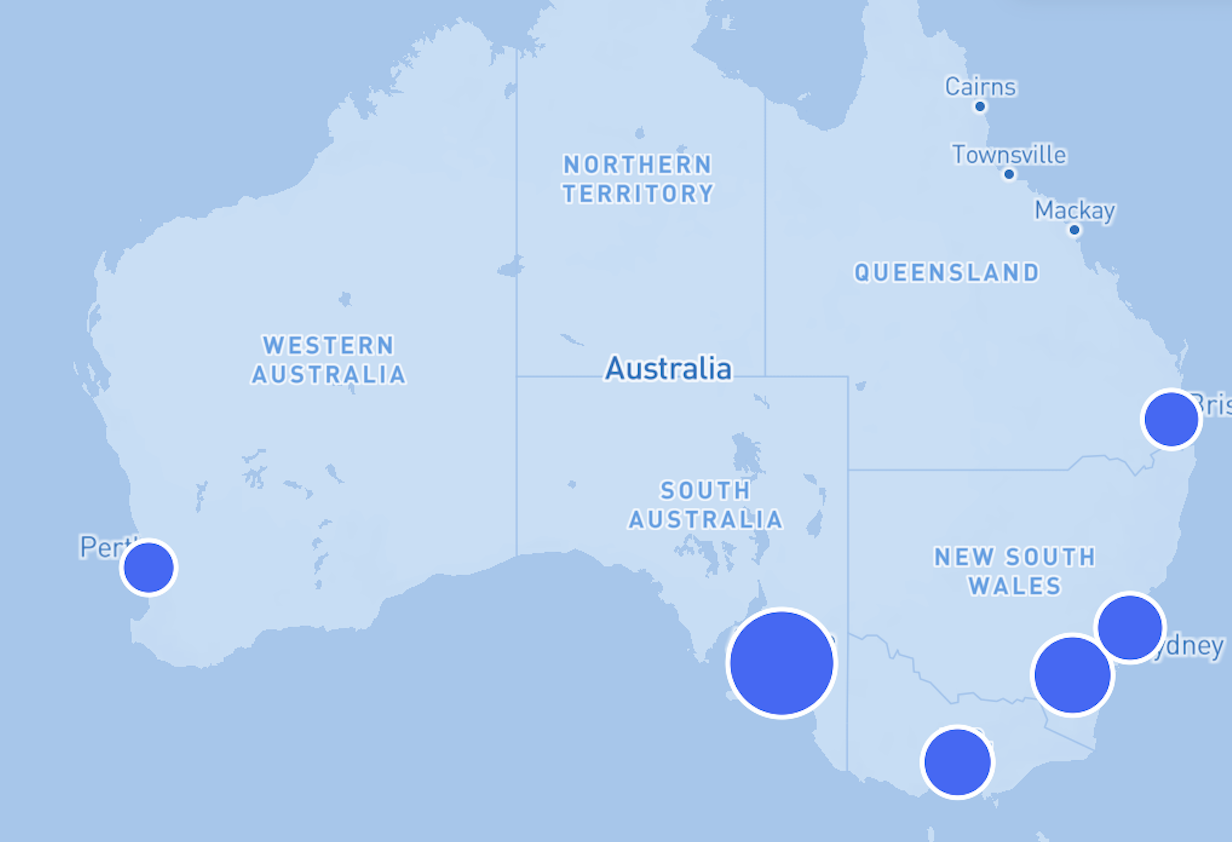
\includegraphics[width=3.5in]{Figures/Screen Shot 2021-05-25 at 8.47.44 pm.png}}
\caption{Map\label{map}}
\end{figure}

\begin{figure*}[h!]
\centering
\begin{minipage}[t]{0.48\textwidth}
\centering
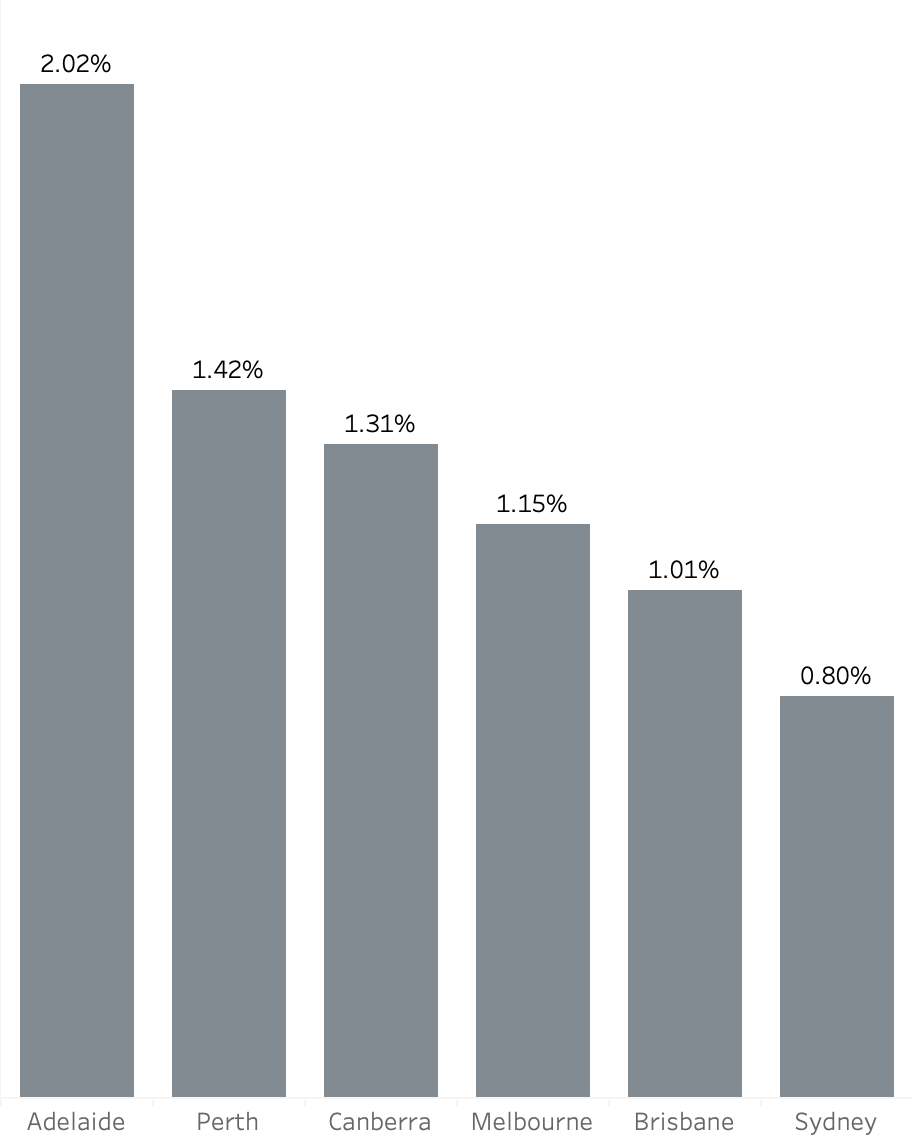
\includegraphics[width=8cm]{Figures/sports rate.png}
    \caption{Sports Tweets Ratio}
    \label{fig:sports ratio}
\end{minipage}
\begin{minipage}[t]{0.5\textwidth}
% \hspace{-2cm}
\centering
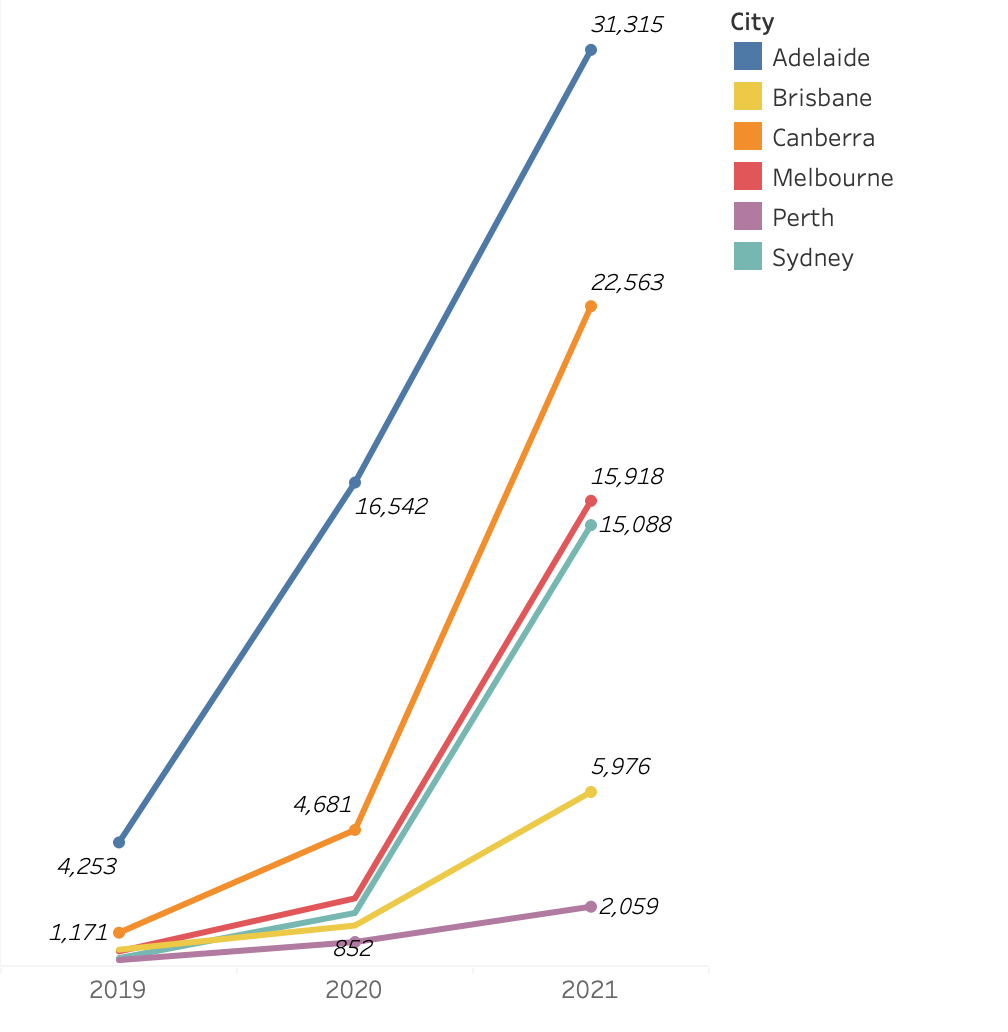
\includegraphics[width=9cm]{Figures/2019-2021.png}
    \caption{Sports Tweets since 2019}
    \label{fig:sports tweets since 2019}
\end{minipage}
\end{figure*}

\begin{figure*}[h!]
\centerline{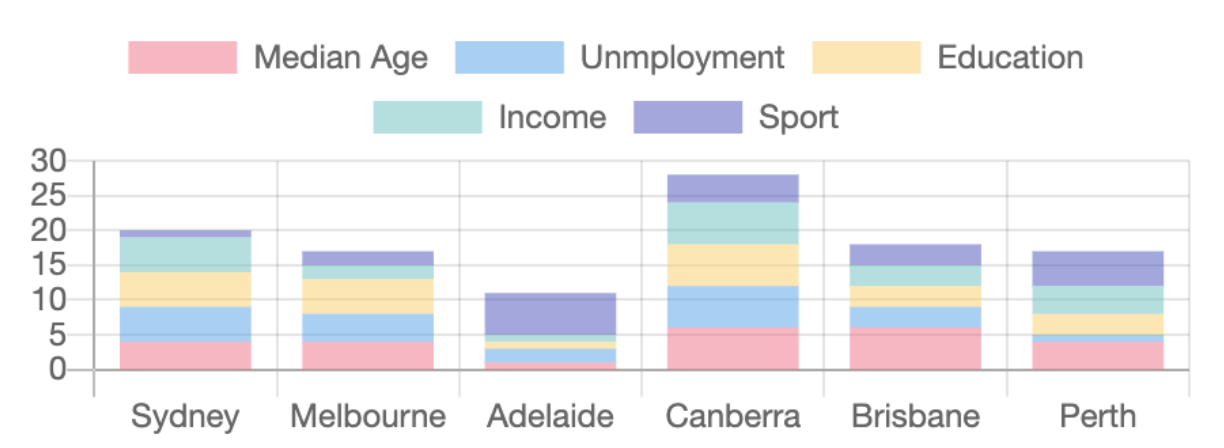
\includegraphics[width=4in]{Figures/vibrant city.png}}
\caption{The Vibrant Cities\label{vibrant result}}
\end{figure*}

According to the 6 factors (gender, age, income, unemployment, education, and sports tweets) discussed above, Canberra wins the most vibrant city (Figure \ref{vibrant result}), as it has earned the most points. This is followed by Sydney and Melbourne, while Adelaide ranked the least in this part.

\subsubsection{Scenario 2: Popular sports}
Assuming the higher the number of sport-related tweets is, the more popular the sport is. During this sports analysis, Twitter data is used to identify the most popular sports across Australia as well as each city respectively. 

\paragraph{CouchDB MapReduce and Django view}
This map function of the CouchDB view is the same one as we showed above. 75 \mintinline{python}{emit ()} functions are used to create entries for each type of sports tweet, and only the mentioned sport in the tweet returns 1. Then the reduce function \mintinline{python}{_sum} is used to summarize the total number for each sport. However, in the Django view, we do not need to sum up all sports results for each city. Instead, the Django REST framework returns each sports popularity result for each city, as well as for all cities. This can be done by writing Python in Django view.

\paragraph{result}
\begin{figure*}[h!]
\centerline{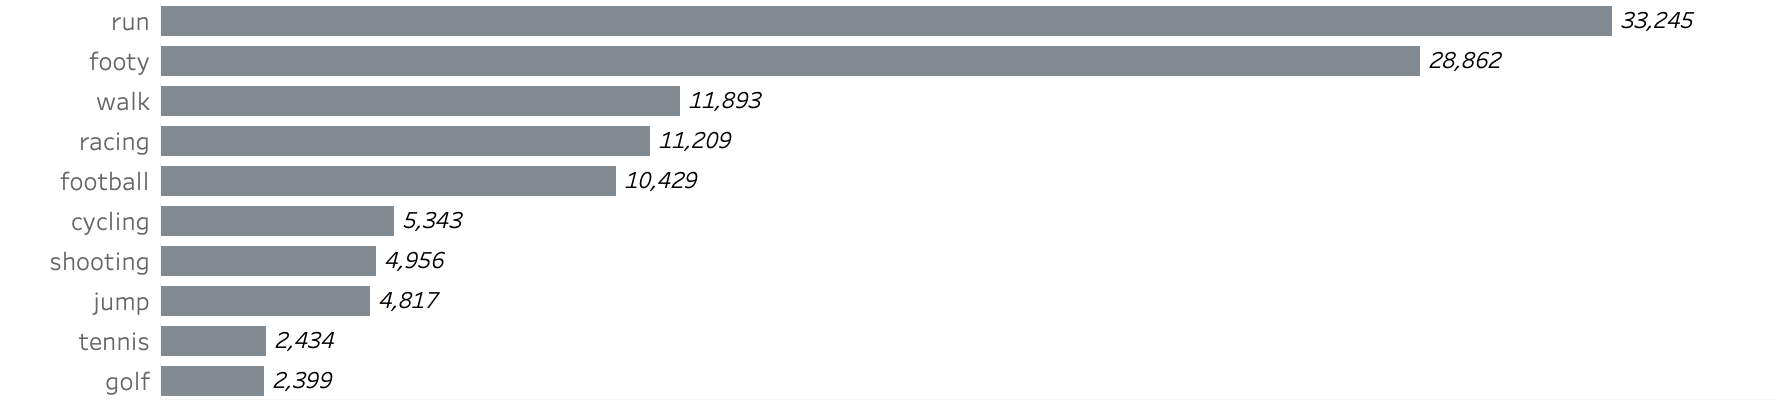
\includegraphics[width=6in]{Figures/popular sports.png}}
\caption{Top 10 Popular Sports  \label{popular sports}}
\end{figure*}

\begin{figure*}[h!]
\centerline{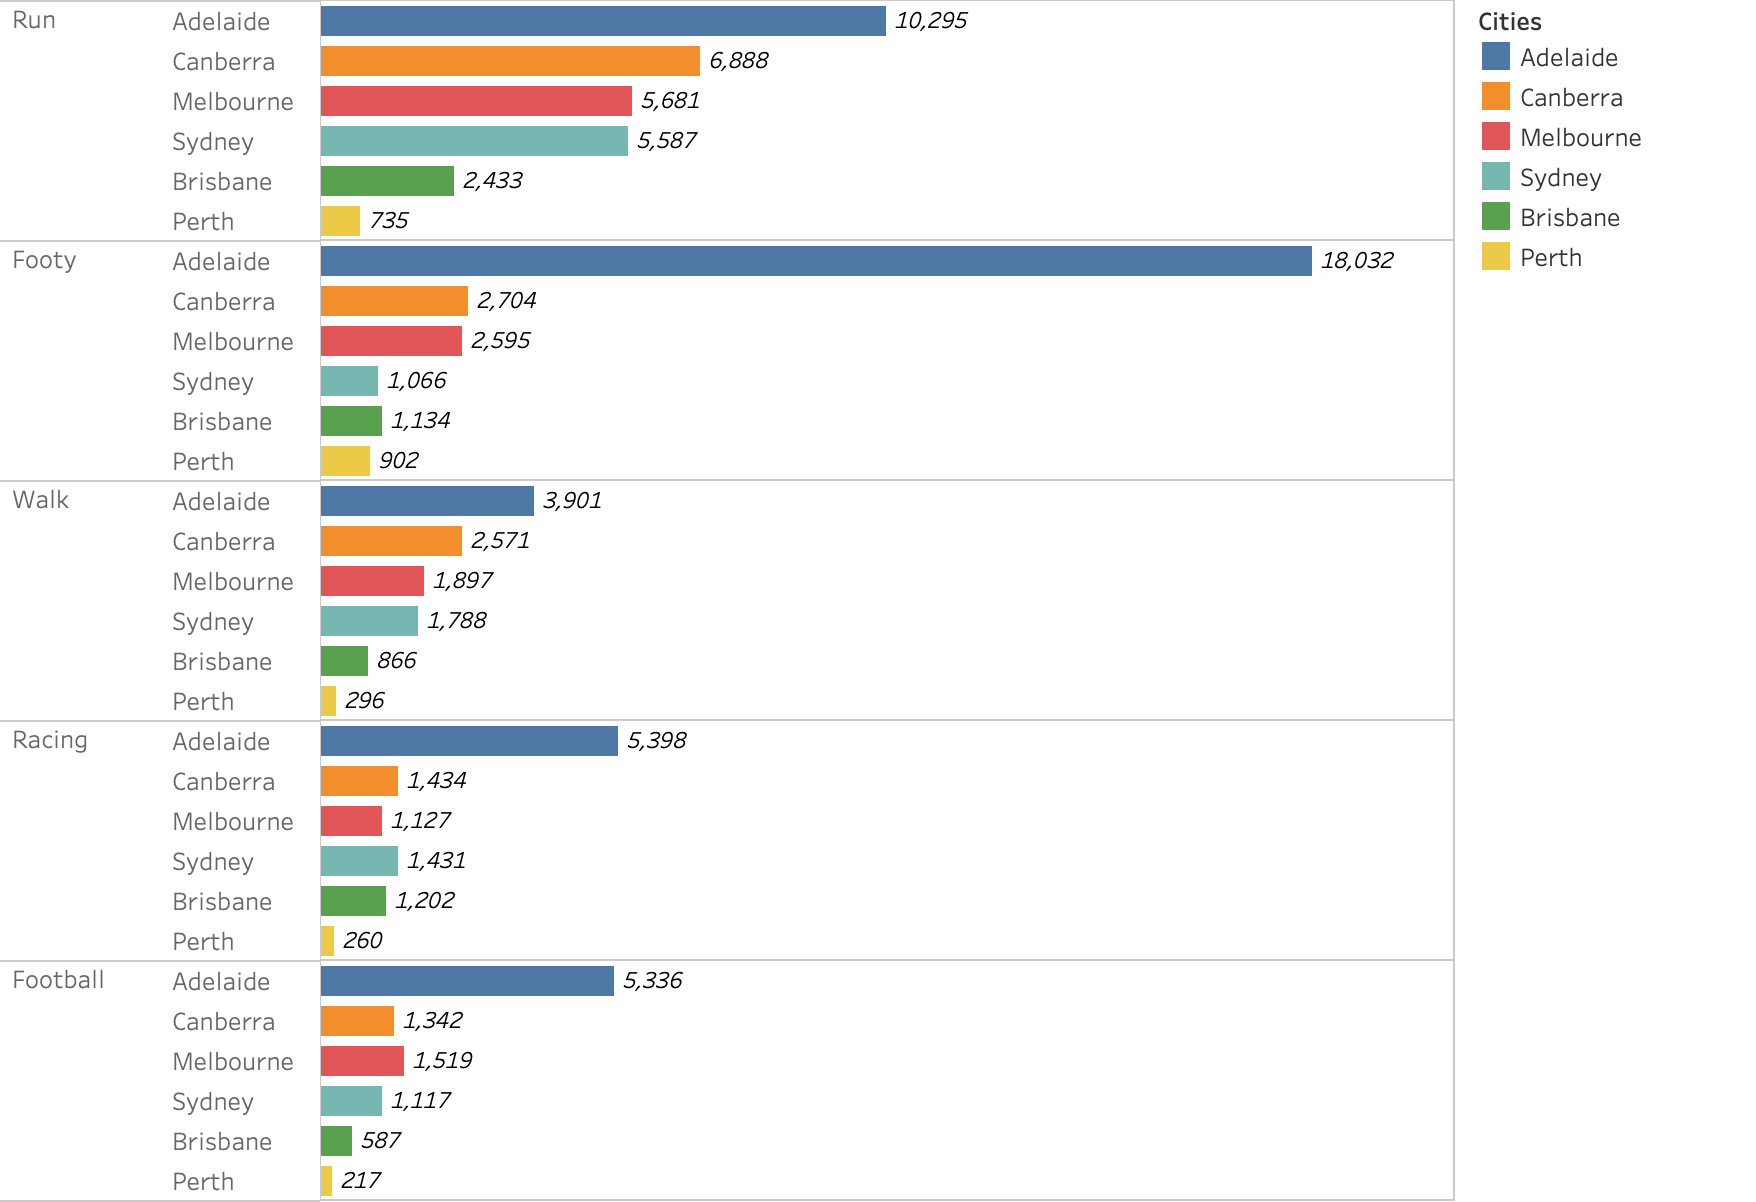
\includegraphics[width=6in]{Figures/popular sports summart.png}}
\caption{Top 5 Popular Sports of each City \label{popular sports of each city}}
\end{figure*}

Among all the sports included in our sports list, “run” is the most tweeted sport among six cities, with over 33,000 related tweets. Next comes to footy, whose number of related tweets is more than twice as "walk", "racing" and "football". "cycling", "shooting", "jump", "tennis" and "golf" whose related tweets rank from a 6 to 10, with the number under 6,000 (Figure \ref{popular sports}).

Twitter user from those six state cities shows the similar preference regarding top 5 sports ("run", "footy", "walk", "racing" and "football"), which are all outdoor activities. While users in Adelaide and Perth discussed "AFL" the most, and people in the other three cities tweeted "run" the most (Figure \ref{popular sports of each city}). 


\subsubsection{Scenario 3: Fitness enthusiasts}
Comparing to the first two scenarios, this one focuses on Twitter users. When it comes to identifying a fitness enthusiast, two factors are considered here, namely, the frequency of posting sports tweets, and the tough level of these sports. Since reducing function in CouchDB cannot be self-defined, we use MapReduce from both CouchDB and Spark to spot the top bodybuilders across the cities. 

\paragraph{CouchDB MapReduce}
MapReduce in CouchDB is used first to return the sports score of each tweet, which is the sum of difficulty points of sports mentioned in the tweet. Meanwhile, the tweet without any sports keywords is removed.  When it comes to a sport that appears in the tweet, the sports score is calculated in the map function by matching sport to related score by using Prototype. In this case, the reduce function used is \mintinline{python}{_count}, and each entry returns a username and sports score. After that, the initial result from the CouchDB view is passed to Django, which then submits the job to Spark.

\begin{lstlisting}[language=JavaScript, caption= Map Functions for Sports Score, backgroundcolor = \color{white}]
function (doc) {
//challenge scores from 75 to 1
 let scoresArr = [75, 74, ..., 2, 1]; 
 
//75 sports array
 let sportsArr=[`boxing', `hockey', ..., `jog']; 
 var score = 0;
 
//get index of challenge score of a sport
 Array.prototype.indexValue=function(arr){
  for(var i=0;i<this.length;i++){
 if(this[i]==arr){
 return i;
 }}}
 
 //get score for each tweet
 for(j = 0; j < sportsArr.length; j++){
 if (doc.val.text.includes(sportsArr[j])){
 score += scoresArr[sportsArr.indexValue(sportsArr[j])];
 }}
 
 //return username and sports score 
 if (score>0){
 emit(doc.val.user.name,score);
 }}

\end{lstlisting}

\begin{figure*}[h!]
\centerline{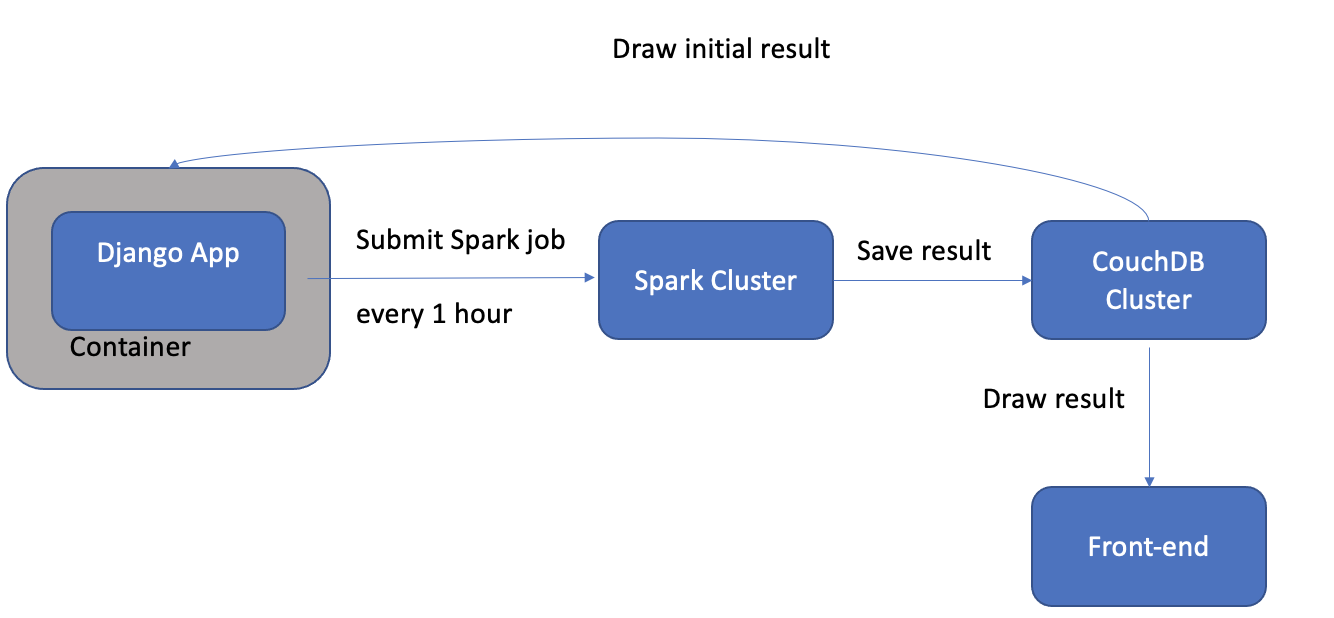
\includegraphics[width=6in]{Figures/couchdb-spark.png}}
\caption{Map Reduce in CouchDB and Spark \label{couchdb and spark}}
\end{figure*}
\paragraph{Spark RDD}
Figure \ref{couchdb and spark} illustrates that the Spark Job, where it aggregates the sports score for each user and sort them by the sport scores in a descending order. The Django application fetches the initial result from the CouchDB view and submits the job to the Spark cluster every hour. Since the top 5 sport enthusiasts does not update frequently, an update frequency of 1 hour is considered adequate for this application. As it does not require user to control, the functionalities remain at a highly usable level. 

\paragraph{Result}
It is interesting that the top 5 fitness enthusiasts' scores are very close, at around 30,000. Specifically, user "Sportageos" is the most hardworking bodybuilder, which is followed by user "Dani Abbracciavento". "Kenny Lu" comes to the third (Figure \ref{enthusiasts}).

\begin{figure}[H]
\centerline{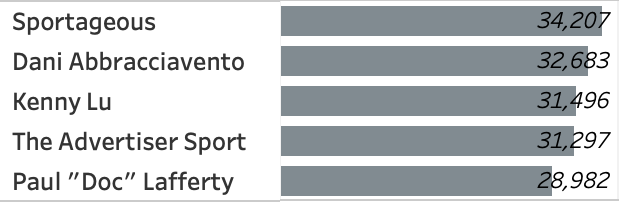
\includegraphics[width=3in]{Figures/enthusiasts.png}}
\caption{Fitness Enthusiasts \label{enthusiasts}}
\end{figure}

\subsection{Future work}
Two things were planned for future implementation.
The first one is to expand the number of cities in this application. Due to the limitation of the project timeframe and lack of data related to cities, we only analyzed and presented the data of six cities in this project. However, we designed a highly scalable backend that allows us to expand the number of cities. The procedure consists of three steps. The data and geo-locations of a new city can be firstly added into the Aurin database and the City database. After adding the data, the tweets of the city can be searched and stored by instances in MRC since the instance was designed to harvest tweets from cities in the city database. Lastly, if the tweets were stored in the Twitter database, the data can be extracted and analyzed.
 
The second future direction is implementing more scenarios and doing natural language processing. In this project, all three scenarios we analyzed mostly required keywords, so the contents of tweets were not analyzed in another aspect. However, in the future, we can provide more scenarios, for example, checking the kinds of sports that most people like or dislike. These scenarios can be presented by doing sentiment analysis on tweet contents. The analyzing process can be easily achieved since all tweet contents were already stored in the database.


\section{Conclusion}

By the time this report is composed, 44,774 users and 10,535,184 tweets have been collected and stored in CouchDB. It is proved that the parallel Twitter harvester gathers data faster than a single program. High scalability is achieved by the use of Docker Swarm, where scaling and deployment become relatively simpler tasks. Ansible enables the system to be deployed with a one-time execution of a shell script. The job control system enables the user to continue the harvesting, which is well-fitted with the highly usable scale tools in the system. 

The data were analysed using both CouchDB MapReduce and Spark RDD. The conclusions are passed to the front-end by Django and JavaScript for visualisation. The results are embodied in three scenarios. The first one is identifying the most vibrant city, and it turns out Canberra is the winner, with the youngest median age(36 years), highest income(1000 dollar per week), highest education rate, and lowest unemployment rate (5\%). The second scenario is the most popular sports. By aggregating the related sport, top 10 sports are found, which are running, footy, walking, racing, and football, etc. The last scenario is the sport enthusiasts rank, with top 5 body builders are picked out. 

\section{Appendix}

\subsection{URLs}
Project Links: 

\href{https://bitbucket.org/comp90024team39/comp90024-a2/src/master/}{Bitbucket Repository}

(https://bitbucket.org/comp90024team39/comp90024-a2/src/master/)

\href{https://youtu.be/574I-g7GSGI }{Production Deployment Video} 

(https://youtu.be/574I-g7GSGI )

\href{https://youtu.be/cqmxZdLdOyk}{Product Demo Video} 

(https://youtu.be/cqmxZdLdOyk) \\

This application supports following URLs:
\begin{itemize}
    \item Page navigation: \url{http://172.26.129.79/analyser/}
    \item Tweets related: \url{http://172.26.129.79/analyser/tweets/}
    \begin{itemize}
        % \item Get single tweet:\\ \url{http://172.26.129.79/analyser/tweets/:id}
        \item Get the stats of tweets\\
        \url{http://172.26.129.79/analyser/tweets/stats/}
        \item Get the stats of sport related tweets\\
        \url{http://172.26.129.79/analyser/tweets/sports}
    \end{itemize}
    \item User related: \url{http://172.26.129.79/analyser/users/}
    \begin{itemize}
        \item Get stats of users\\
        \url{http://172.26.129.79/analyser/users/stats}
        \item Get the sport enthusiasts rank\\
        \url{http://172.26.129.79/analyser/users/rank/}
    \end{itemize}
    \item Sport related: \url{http://172.26.129.79/analyser/sports/}
    \begin{itemize}
        \item Get the stats of sports\\
        \url{http://172.26.129.79/analyser/sports/stats_all}
        \item Get the stats of sports in specific yearly time interval (from 2019 to 2021)\\
        \url{http://172.26.129.79/analyser/sports/<year>-<year>}
        For example: \url{http://172.26.129.79/analyser/sports/2019-2020/}
        \item Get the top 3 sports\\
        \url{http://172.26.129.79/analyser/sports/rank_top3}
    \end{itemize}
    \item Job control: \url{http://172.26.129.79/analyser/jobs/}
    \begin{itemize}
        \item Get all jobs status\\
        \url{http://172.26.129.79/analyser/jobs/all/}
        \item Start twitter harvester\\
        \url{http://172.26.129.79/analyser/jobs/search}
        \item Start updating users timeline\\
        \url{http://172.26.129.79/analyser/jobs/update}
        \item Start streaming tweets\\
        \url{http://172.26.129.79/analyser/jobs/stream}
        \item Get the sport enthusiasts rank\\
        \url{http://172.26.129.79/analyser/jobs/user_rank}
    \end{itemize}
    \item Initialise couchdb
    \url{http://172.26.129.79/analyser/initialiser}
\end{itemize}

\subsection{User Guide}

This section describes the testing steps. 

\subsubsection{Logins}

CouchDB: user:pass

Portainer: admin:password

HAProxy: admin:password

\subsubsection{Installation}

\textbf{To install the system: }

\begin{itemize}
    \item Clone the repository and change directory to $./deployment$.
    \item Prepare a clean project unimelb-comp90024-2021-grp-39 on MRC. if you want to use other projects, update unimelb-comp90024-2021-grp-39-openrc.sh content with your openrc.sh code. 
    \item Run \href{https://bitbucket.org/comp90024team39/comp90024-a2/src/master/deployment/init.sh}{./init.sh}
    \item enter the password from MRCpassword.txt or your own. 
    \item Go to the home page (any instance IP)
    \item Go to Manage
    \item Set up as local swarm
\end{itemize}

\\

\textbf{To scale up instances,}

\begin{itemize}
    \item Inspect \href{https://bitbucket.org/comp90024team39/comp90024-a2/src/master/deployment/host_vars_scale.yaml}{./host\_vars\_scale.yaml} and update the details of the new resources
    \item Run \href{https://bitbucket.org/comp90024team39/comp90024-a2/src/master/deployment/init.sh}{./scale.sh}
    \item Enter the master password from MRCpassword.txt or your own
    \item Go to the home page (any instance IP) 
    \item Go to ``Manage" from the bottom left of home.
    \item Portainer login is admin:password. 
    \item Go to Services 
    \item Scale up services by an appropriate level.  
\end{itemize}

\\

\textbf{To scale up services,} 
\begin{itemize}
    \item Go to Manage page (Portainer) from home
    \item Go to Services 
    \item Click Scale
    \item Enter the number of nodes
    \item click tick
\end{itemize}

An important note is that CouchDB ideally needs at least 2 cores to run properly, as mentioned by its developer. \\

\textbf{To check where the containers are distributed: }

\begin{itemize}
    \item Go to Manage page (Portainer)
    \item Go to Dashboard 
    \item Click ``Go to the visualizer"
\end{itemize}

\subsubsection{Testing}

If charts are missing on the Statistics page, please refresh the page and the charts will load. 

\textbf{To test the harvesters,}

\begin{itemize}
    \item Enter the number of users per city on the home page bottom panel
    \item Click Add New Users
\end{itemize}

The more users exist in the database, the harder it is to get new users. Typically a batch job of 1 new user per city consumes 15-30 minutes to finish.\\

\textbf{To add more tweets,}

\begin{itemize}
    \item Click Search User Tweets
\end{itemize}

Normally this will search for the user timeline for all the users who have not been harvested for over 7 days. Since a lot of user data were collected early, this job will run for a long time. The tester may need to wait 10-20 minutes to see the first update. 

Moreover, the tokens being used might be limited at this stage since the beginning, so the wait time on new data collection is not guaranteed. 

When stopping the jobs, it may take a few minutes to completely stop. 

We had planned to partition the database by cities, but only realised the 10G partition size limitation when most data is in place. It is estimated to take 2 days to migrate the partition method and the relevant code. It is not a difficult job but CouchDB will consume 10-15 hours to rebuild the views. Due to the limited time-frame, we have left it as is. If the user continues to harvest a large amount of data, it may potentially hit the size limit. 


\subsubsection{Troubleshooting}

If CouchDB services are restarted or you see ``Failed to load database" error run \href{https://bitbucket.org/comp90024team39/comp90024-a2/src/master/deployment/recluster-couchdb.sh}{recluster-couchdb.sh} 

\subsubsection{UI}
Home page (Fig.\ref{UserGuid1}, \ref{UserGuid2} link: \url{http://172.26.129.79/home/}): On the left side is the navigator. It is composed by two parts, \textcircled{1} Page Navigator and \textcircled{2} Management Menu. Users can switch to other pages through \textcircled{1}Page navigator for more information extracted from harvest data, admin can manage the instances (\url{http://172.26.129.79:9000}), HAProxy (\url{http://172.26.129.79/haproxy-admin/}), Spark (\url{http://172.26.129.79:8080}) and CouchDB (\url{http://172.26.129.79:5984}) with the \textcircled{2}Management menu. \textcircled{3} Twitter Harvest Status shows the Twitter harvester status in instances. There are two statuses. When the job is running, the status will be displayed as running, and idle means the job is ready to start. Users can start the job with the \textcircled{4} Twitter Harvest Job Control Module. The control buttons will be enabled if the corresponding Twitter harvest status is idle. The search button means searching for new tweets. Before clicking the search button, users need to input the number of users they want to search in the input box. Click the stream button will start harvesting the most recent tweets, and the update button is to update users’ timelines.
\begin{figure*}
\centerline{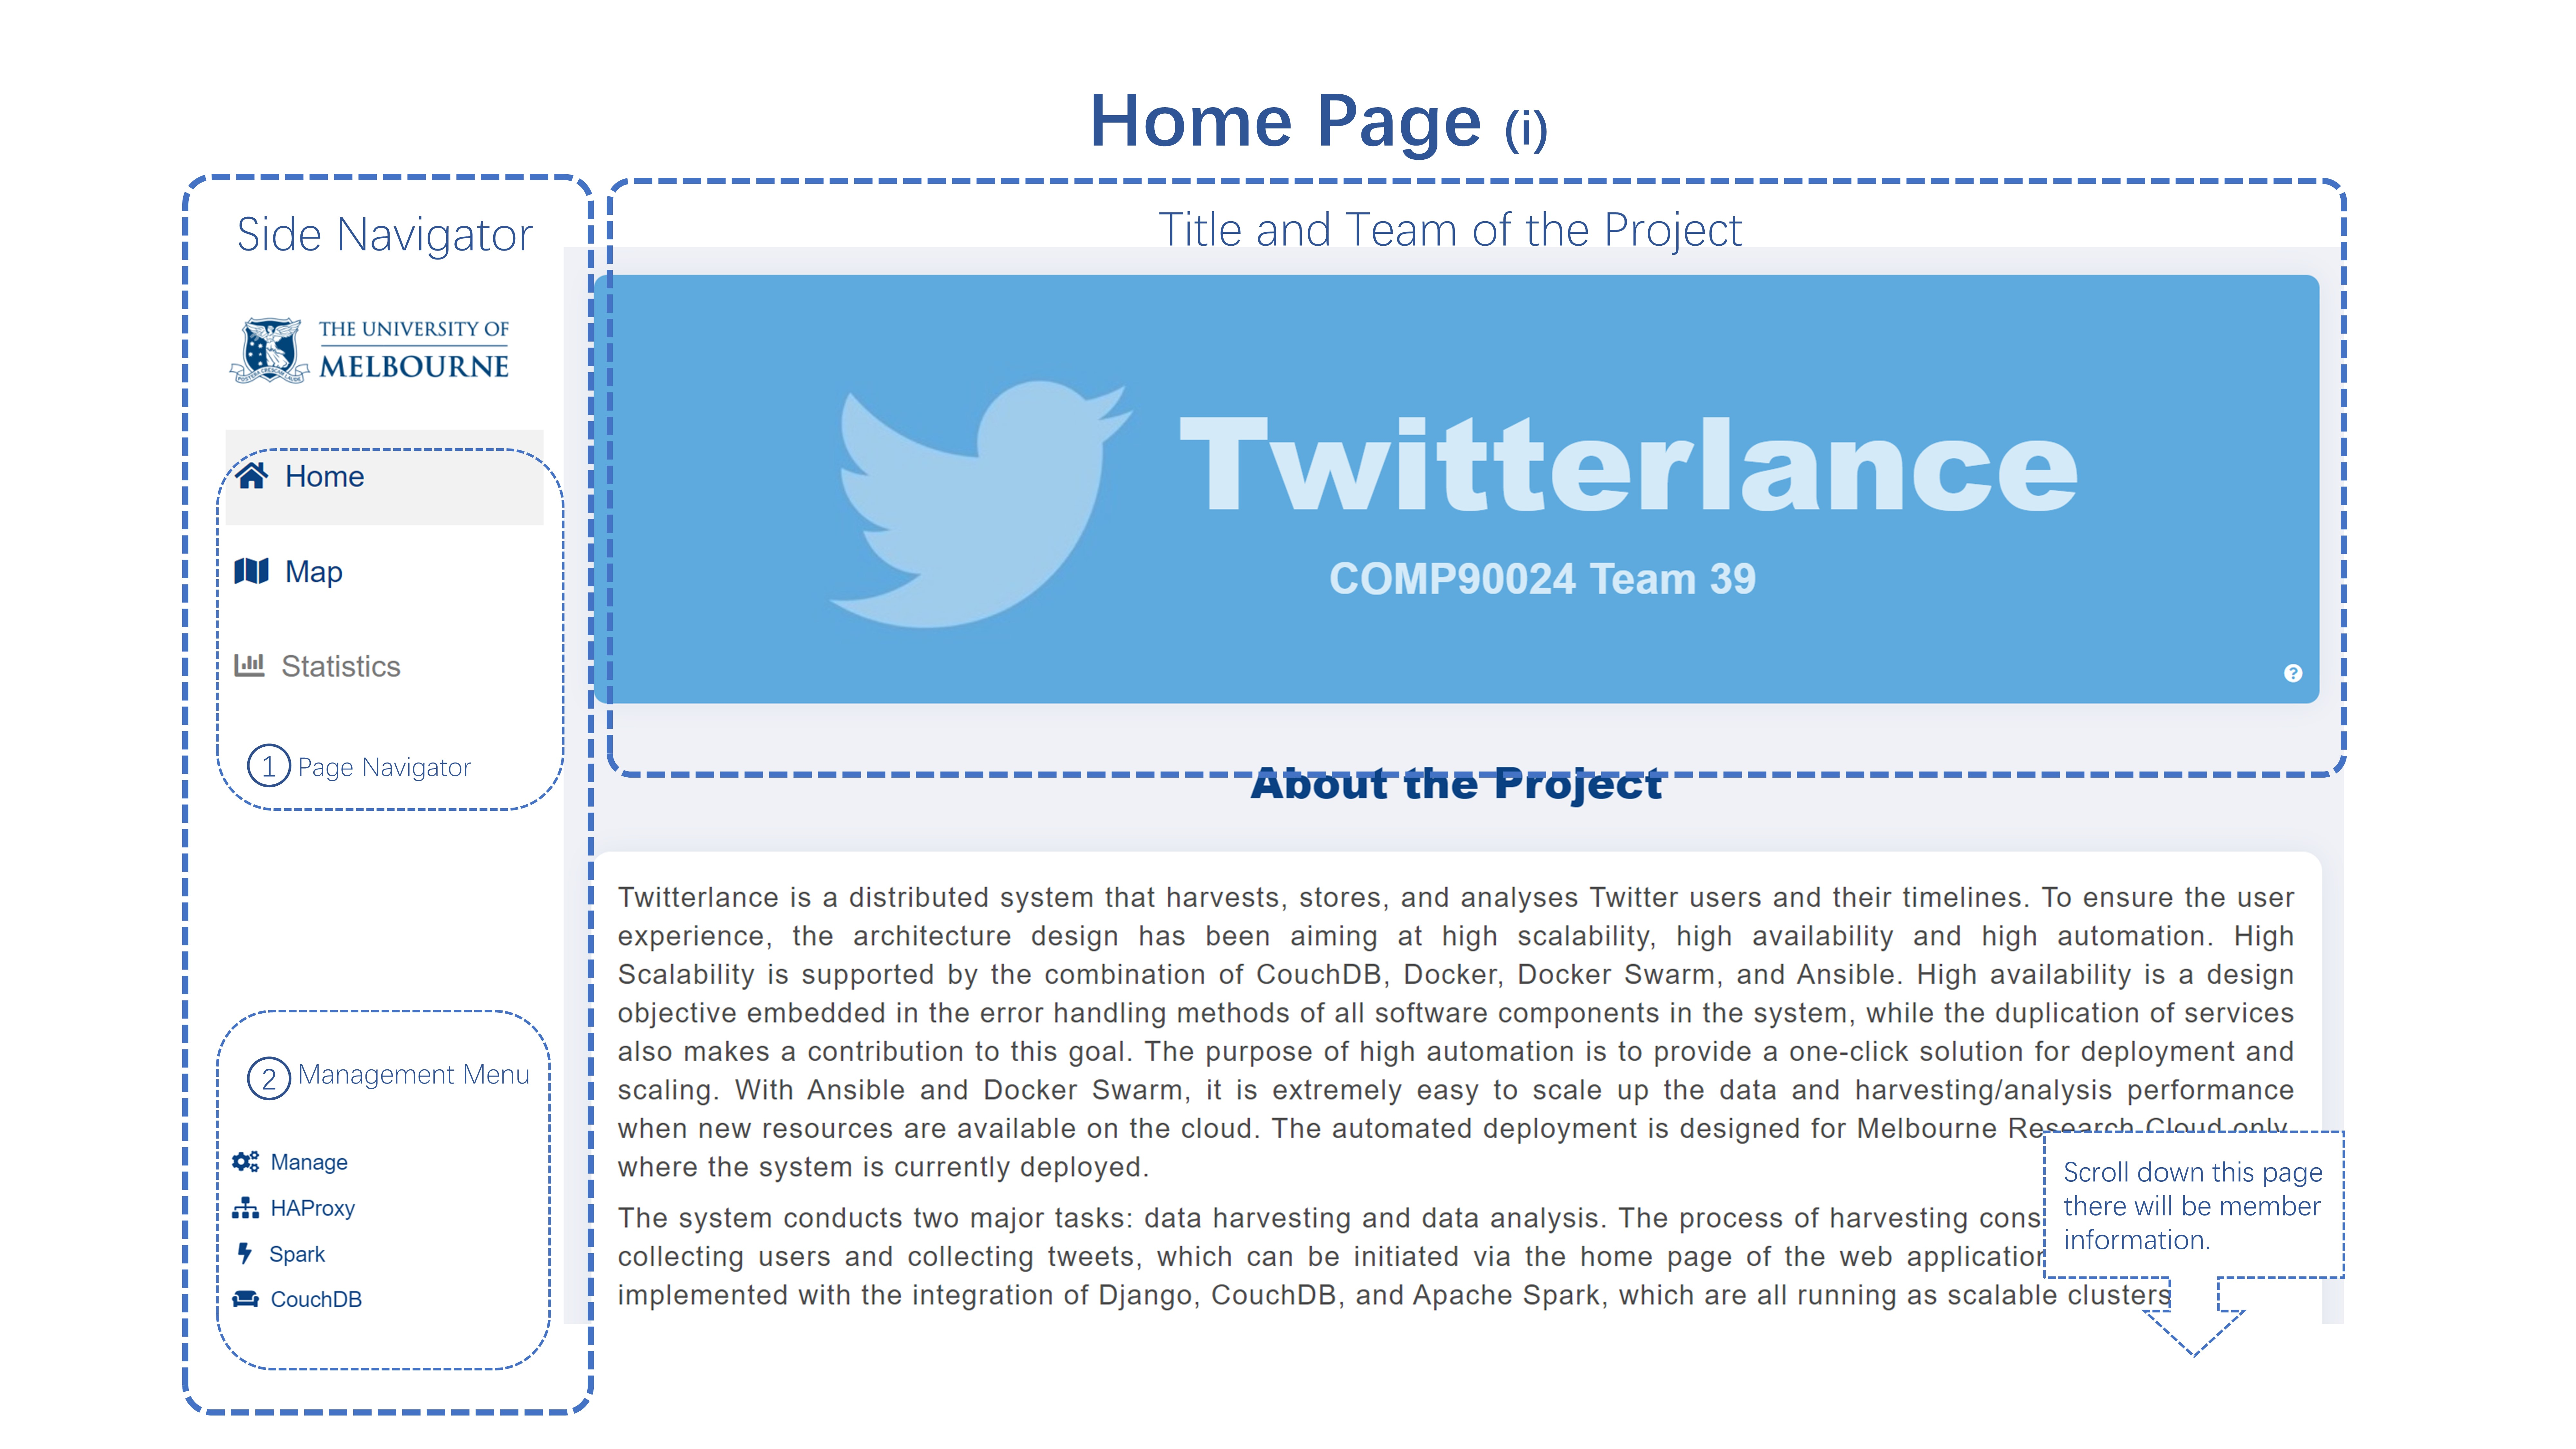
\includegraphics[width=7in]{Figures/UserGuid1.JPG}}
\caption{Home Page (i)}
\label{UserGuid1}
\end{figure*}

\begin{figure*}
\centerline{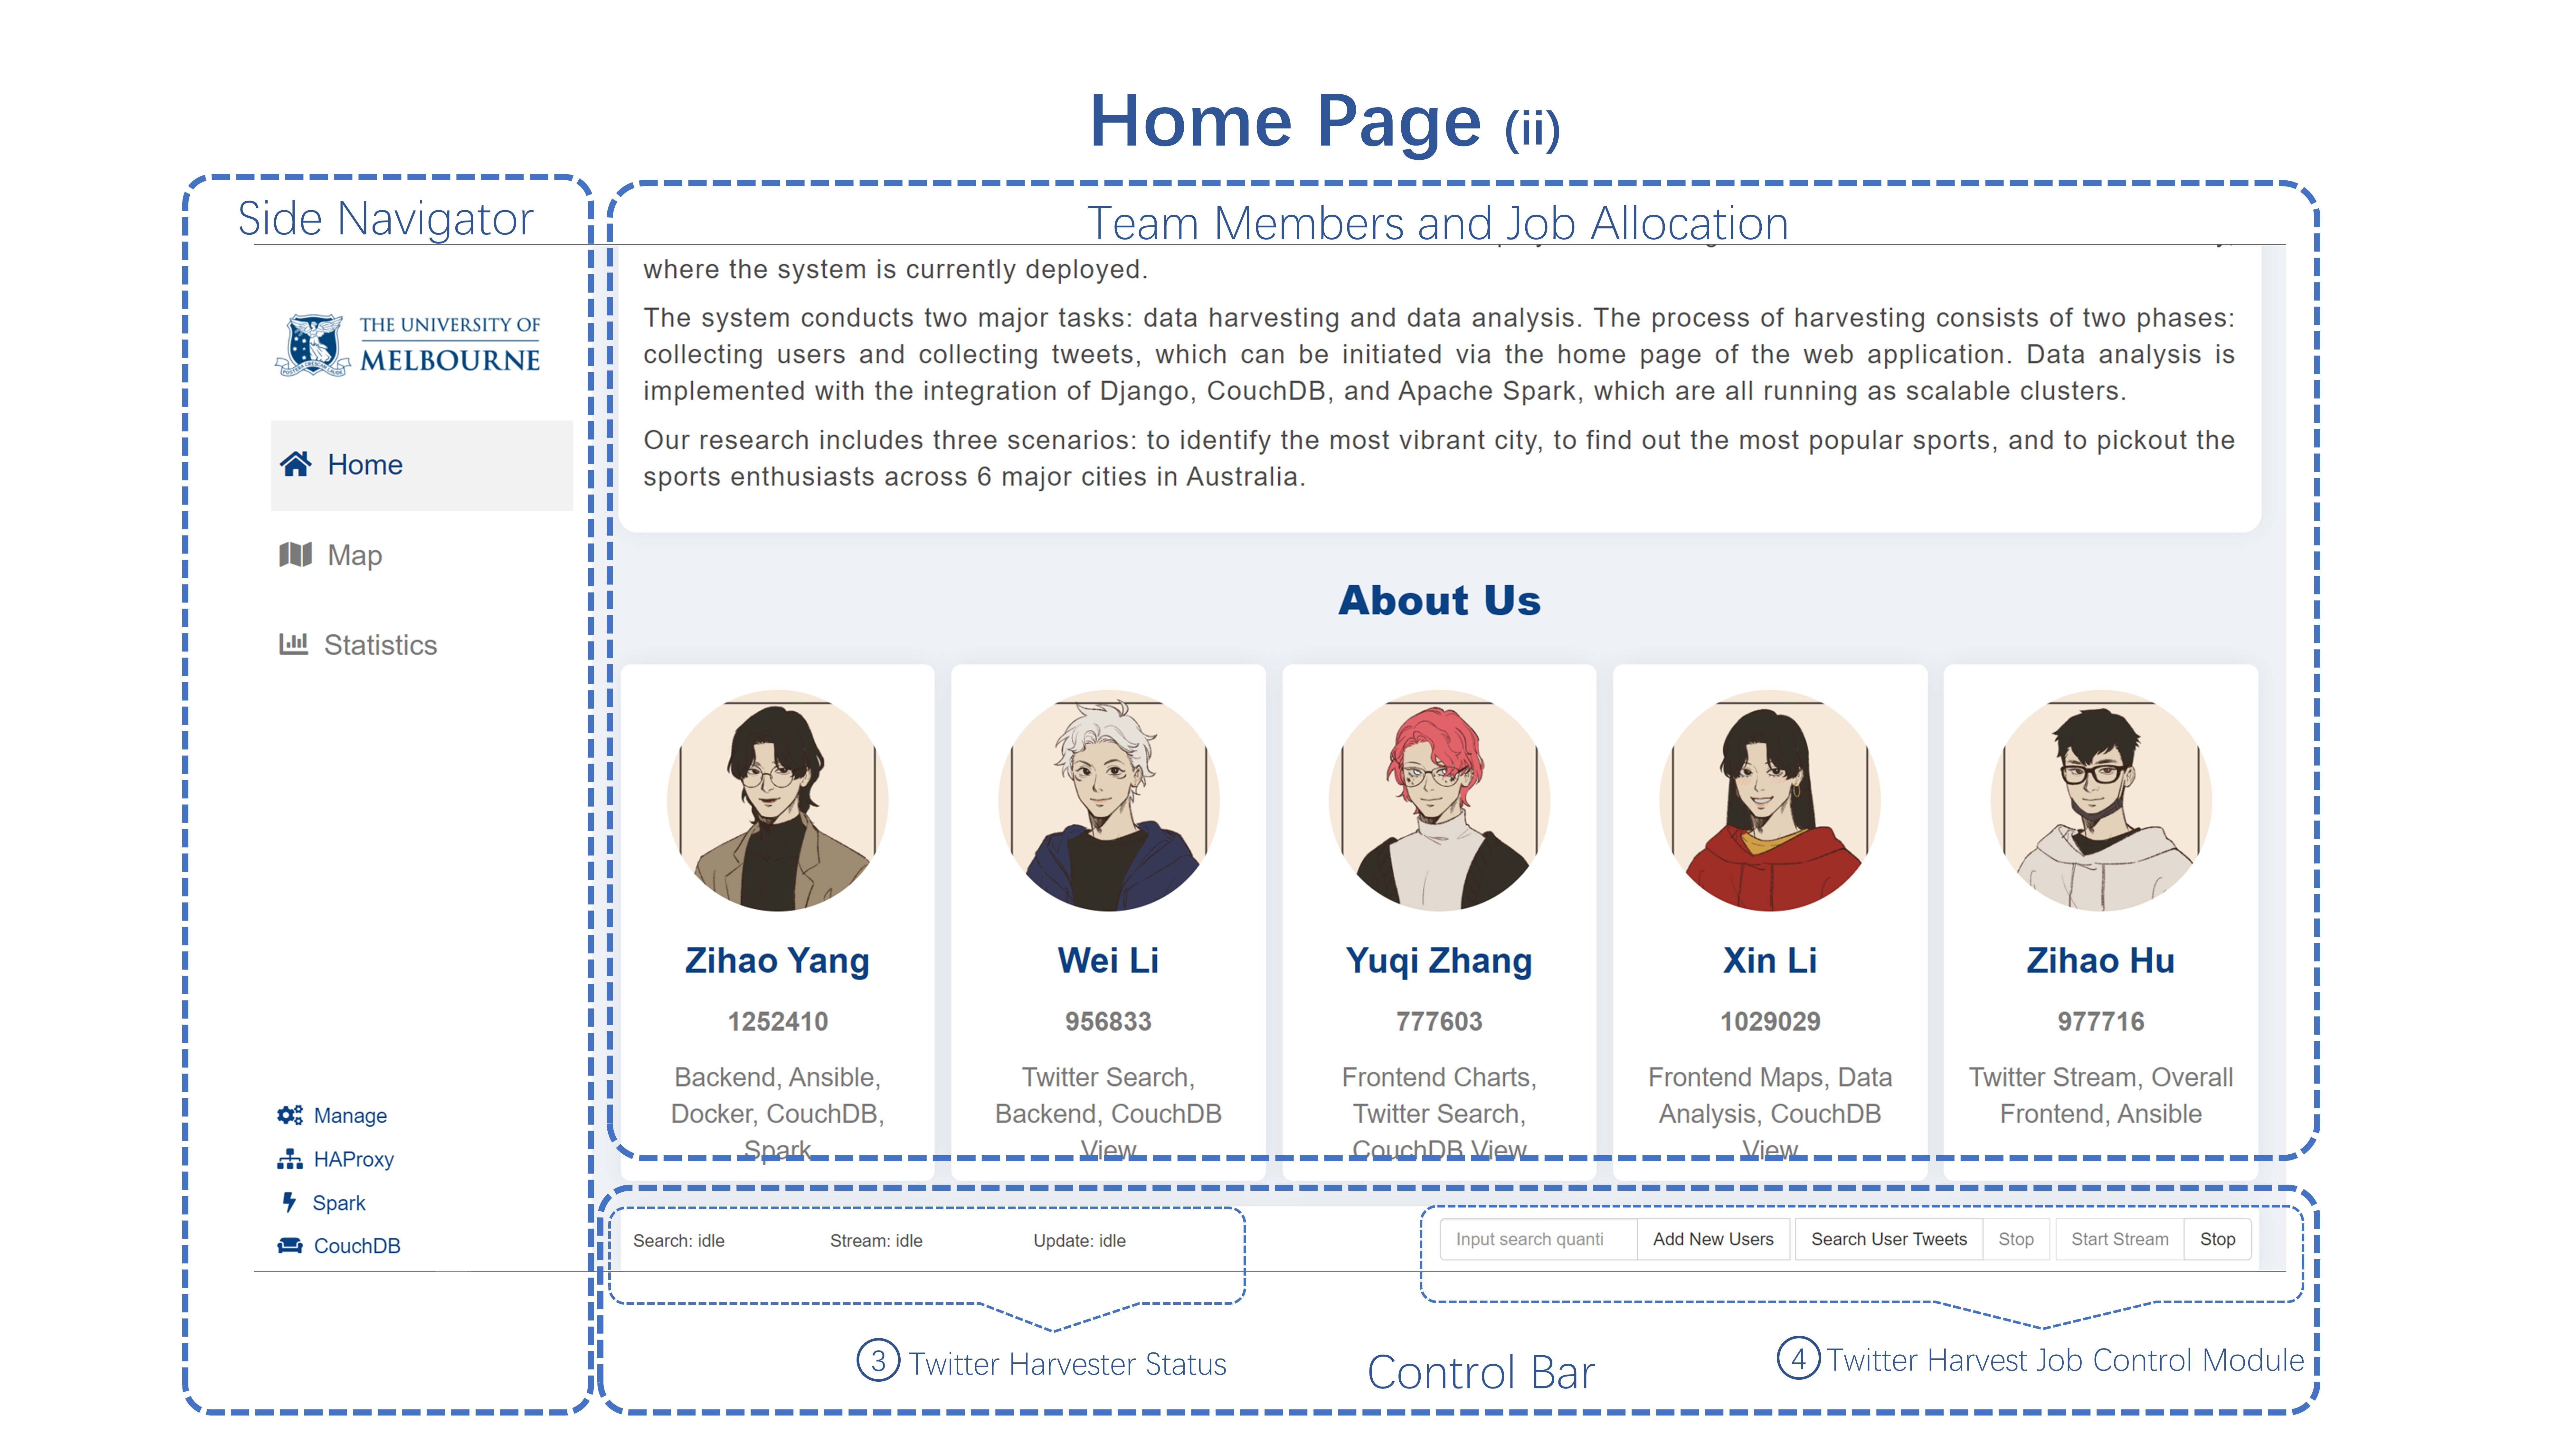
\includegraphics[width=7in]{Figures/UserGuide2.JPG}}
\caption{Home Page (ii)}
\label{UserGuid2}
\end{figure*}

Map page (Fig.\ref{UserGuid3} link: \url{http://172.26.129.79/map/}): Users can quickly locate their interested city with the \textcircled{7} Search Bar on the top right of the page. (For the limit of time and resources we only display data of six cities.) \textcircled{6}Interested Cities will be displayed on the map with blue circles. The radius of circles is decided by the quantities of tweets harvested in corresponding cities. When the mouse hovers on one of the interested cities, \textcircled{5}Statistics of the city will be displayed on the left side of the map page.

\begin{figure*}
\centerline{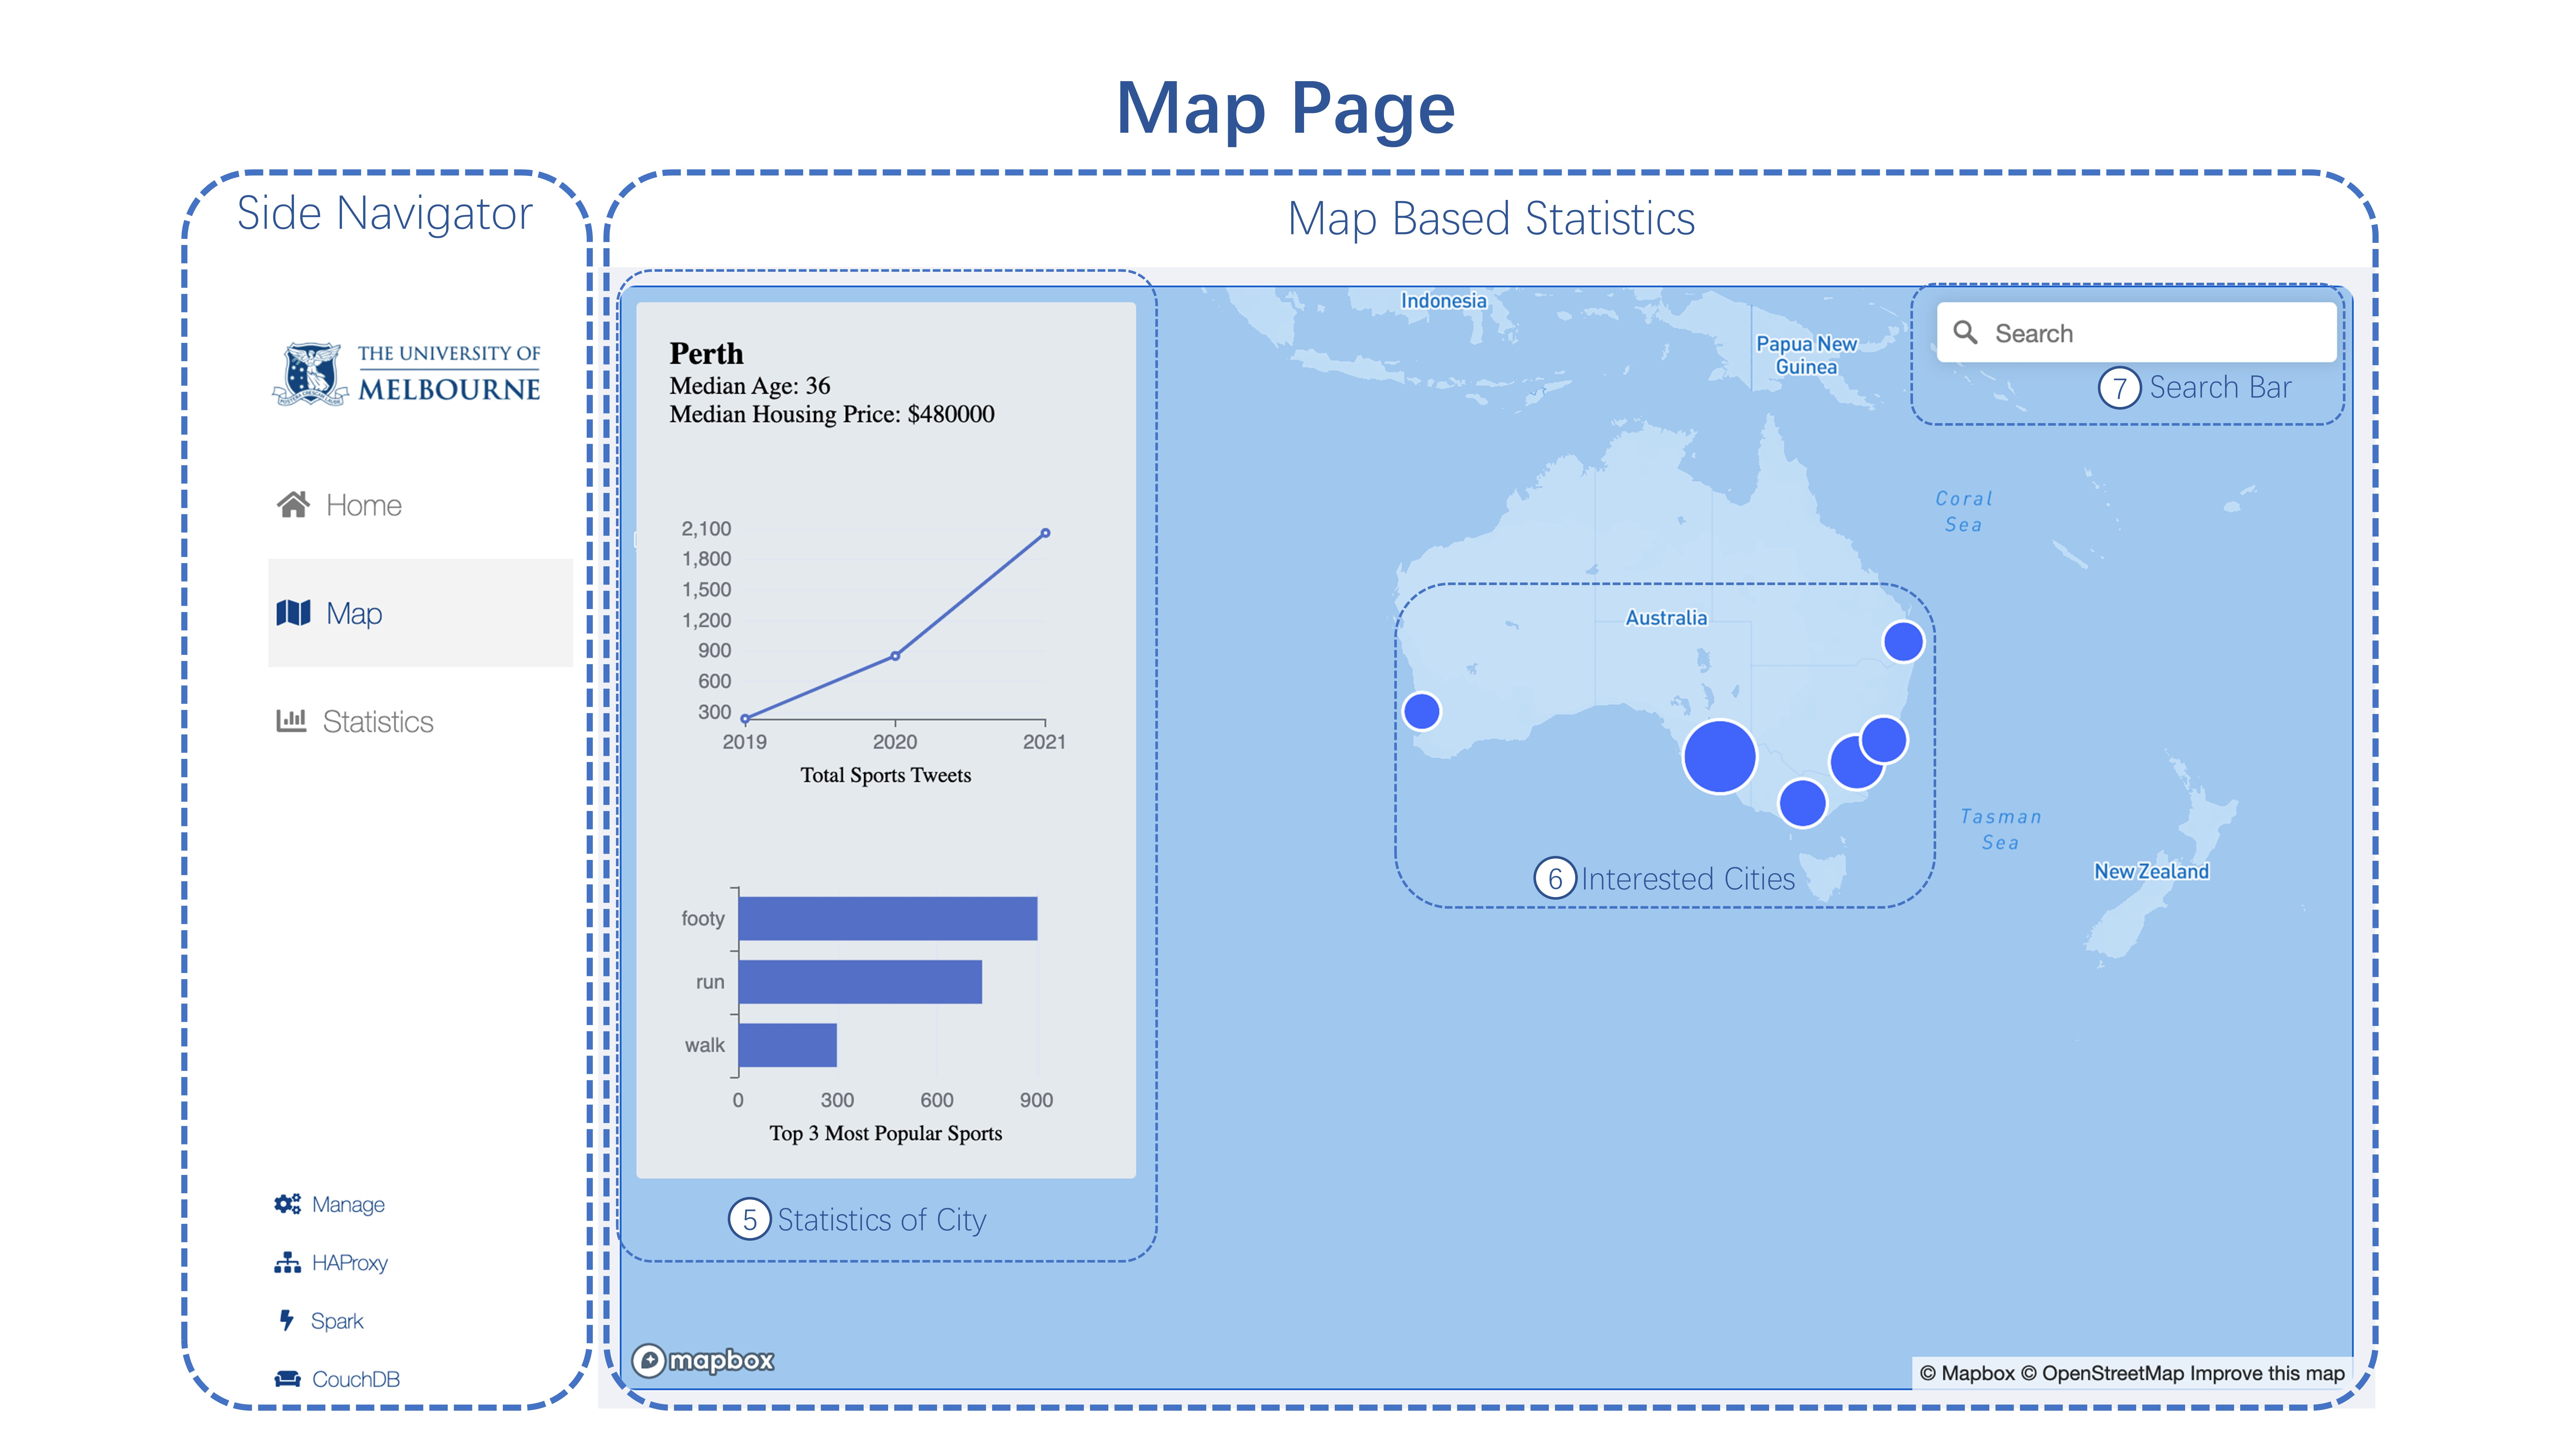
\includegraphics[width=7in]{Figures/UserGuide3.JPG}}
\caption{Map Page}
\label{UserGuid3}
\end{figure*}

Statistics page (Fig.\ref{UserGuid4} link: \url{http://172.26.129.79/statistics/}): \textcircled{8}Overall statistics shows: a) the total number of users we searched and stored in the database, b) the total number of tweets we harvested from users, c) the total number of sport-related tweets. Users can switch to different charts through the \textcircled{9} Chart Tab. When the chart tab is activated, the color will be changed from blue to white. Sex $\&$ Age tab is linked to bar-charts of the gender ratio and median age across six cities. Work $\&$ Study tab is linked to the bar charts of the unemployment rate and Education level across six cities. Income $\&$ Freq tab is linked to the bar-charts of median-income and tweets frequencies across six cities. More scenarios will be displayed if Users scroll down this page.

\begin{figure*}
\centerline{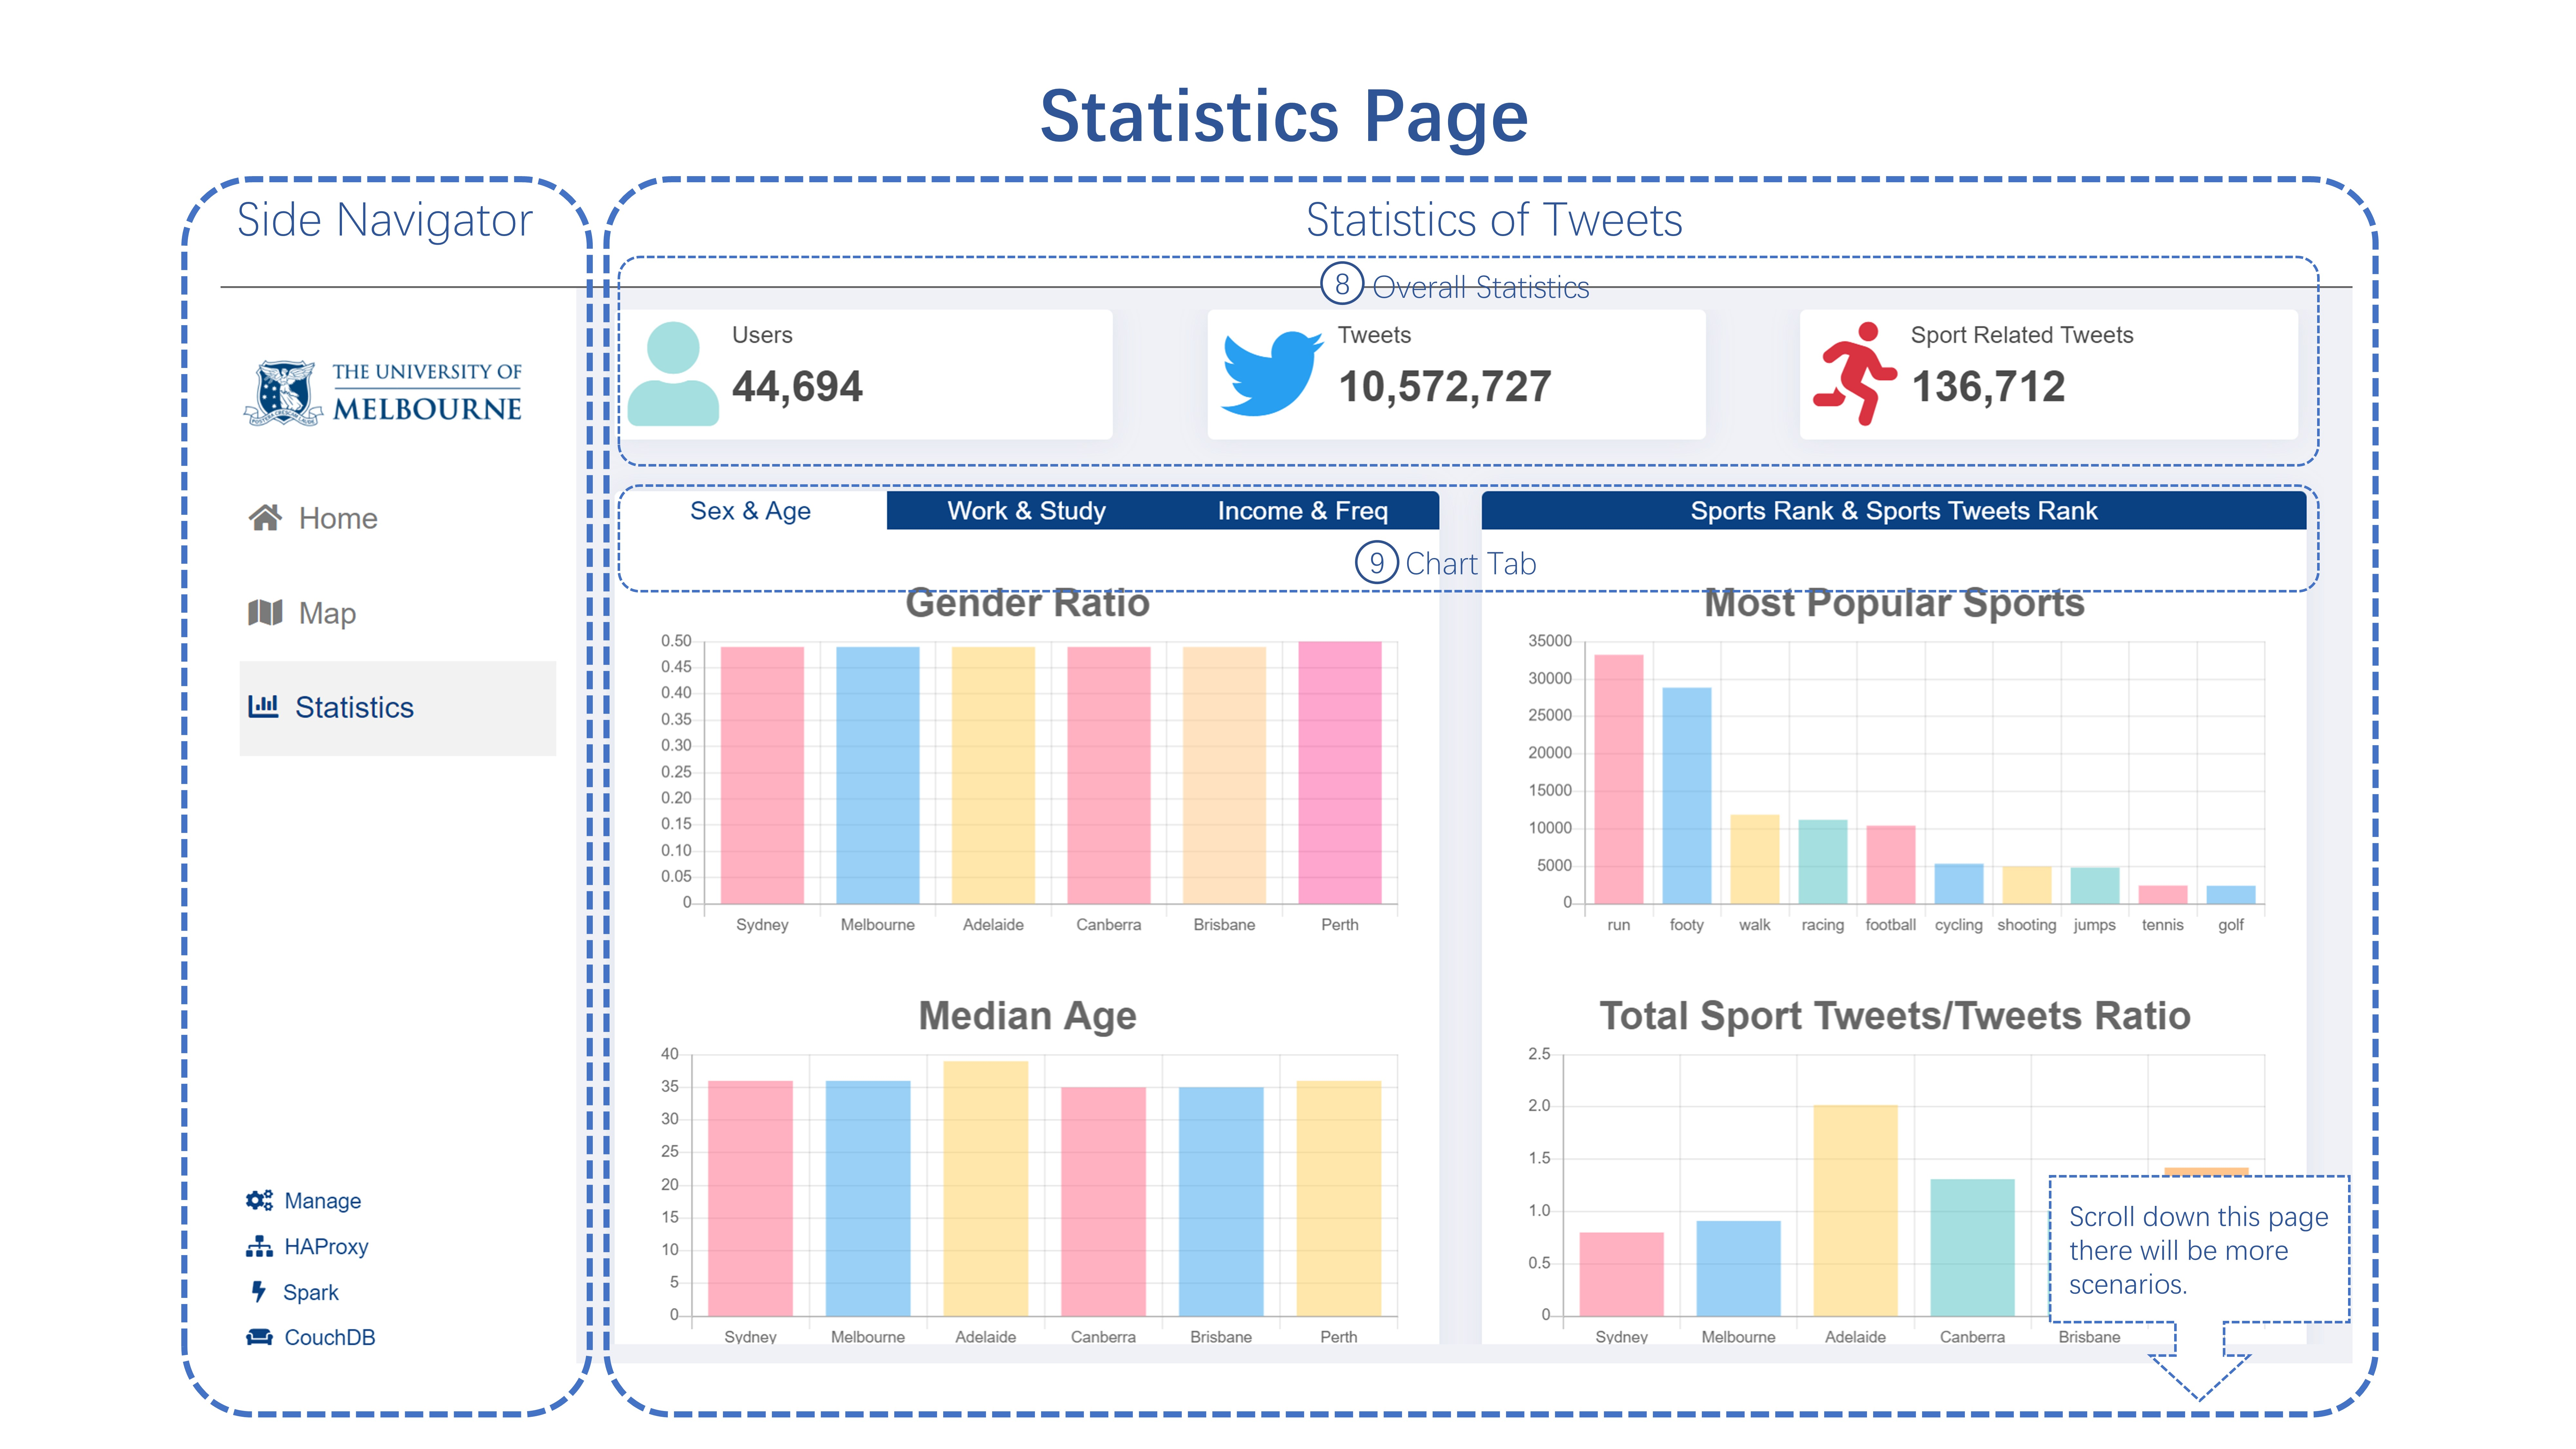
\includegraphics[width=7in]{Figures/UserGuide4.JPG}}
\caption{Statistics Page}
\label{UserGuid4}
\end{figure*}
\newpage

\subsection{Pseudo code}
\begin{algorithm}[h!]
\caption{Search User Algorithm}
\SetAlgoLined
\SetKwProg{Fn}{Function}{}{end}
\SetKwProg{try}{try}{:}{}
\SetKwProg{except}{except}{:}{}
\Fn{search\_user(query: str, city: str, api, rate\_limit = 10, latest\_id = None, count = 0)}{
\tcc{query = whitespace, used in Twitter API}
\tcc{city = the full name of city, used in structure user profile}
\tcc{api = Twitter API token, user in Twitter API}
\tcc{rate\_limit = how many users the system want to add in this city}
\tcc{latest\_id = the oldest tweet index in a batch tweets, used in breakpoint retransmission}
\tcc{count = how many users have been added, used in breakpoint retransmission}
Initiation;\\
get user list from users database in CouchDB;\\
get geocode of the city from cities database in CouchDB;\\
\eIf{Twitter API works}{
pass\;
}{
\KwRet \tcc{move to next token}
}
\While{count does not meet the rate\_limit}{
\try{}{
yield a batch of tweets from search API;\\
}
\except{}{
\KwRet False, maxid, count \tcc{move to next token}
}
\For{tweet in tweets}{
\eIf{the user not in the user list}{
append the user to save list\;
}{
pass
}
}
\try{}{
feed the save list to CouchDB;\\
}
\except{}{
retry for 5 times maximally;
}
\eIf{success to save users}{
get the maxid of that batch;\\
count += the length of the save list;\\
}{
continue in this batch
}
}
\KwRet True, None, count
}
\label{algorithm: searchuser}
\end{algorithm}

\begin{algorithm}[h!]
\caption{Run Search User Algorithm}
\SetAlgoLined
\SetKwProg{Fn}{Function}{}{end}
\Fn{run\_search(i: int)}{
\tcc{i = the rate\_limit fed from the frontend}
get cities from cities database in CouchDB;\\
get tokens from tokens database in CouchDB;\\
scale up and shuffle token list;\\

\For{city in cities}{
\For{token in tokens}{
get api from token list;\\
\eIf{search\_user returns True}{
break}{
continue to search from the returned maxid and count} 
}
}
}
\label{algorithm: runsearch}
\end{algorithm}

\begin{algorithm}[h!]
\caption{Run Update Timeline Algorithm}
\SetAlgoLined
\SetKwProg{Fn}{Function}{}{end}
\SetKwProg{try}{try}{:}{}
\SetKwProg{except}{except}{:}{}
\Fn{assign\_task()}{
\try{}{get user list from users database in CouchDB;\\}
\except{}{try again 10 mins latter} \tcc{wait for database compaction or view regenerating}
get the node list from nodes database in CouchDB;\\
find the index of current node;\\
evenly split the user list by the node number;\\
assign the node with sub\_user\_list corresponding to its index;\\
\KwRet sub\_user\_list
}
\Fn{run\_update()}{
get tokens from tokens database in CouchDB;\\
scale up and shuffle the token list; \tcc{expand the token pool}\\
assign\_task(); \tcc{assign task for one node}\\
\For{user in sub\_user\_list}{
\For{token in tokens}{
get api from token list;\\
\eIf{search\_tweets returns True}{
break}{
continue} 
}
}
}
\end{algorithm}

\begin{algorithm}[H]
\caption{Update Timeline Algorithm}
\SetAlgoLined
\SetKwProg{Fn}{Function}{}{end}
\SetKwProg{try}{try}{:}{}
\SetKwProg{except}{except}{:}{}
\Fn{search\_tweets(user: dict, api, timeline\_limit= 400)}{
\tcc{user = a dictionary, used in Twitter API}
\tcc{api = Twitter API token, user in Twitter API}
\tcc{timeline\_limit = how many new tweets the system want to add}
Initiation;\\
get user list from users database in CouchDB;\\
get geocode of the city from cities database in CouchDB;\\
\try{}{
yield a batch of tweets from search timeline API;\\
}
\except{}{
\KwRet False \tcc{move to next token}
}

\While{the length of save list of does not meet the timeline\_limit}{
\uIf{the length of the latest batch tweets = 0}{
break
}{
}
\uElseIf{the length of the latest batch tweets = 200}{
save the tweets into save list;\\
get the maxid of this batch;\\
\try{}{yield next batch of tweets from search timeline API;}
\except{}{\KwRet False}
}
\Else{
save the tweets into save list;\\
break;
}
}
\try{}{
feed the save list to CouchDB;\\
}
\except{}{
retry for 5 times maximally;
}
\eIf{success to save users}{
\KwRet True
}{
\KwRet False
}
}
\end{algorithm}


\begin{algorithm}[h!]
\caption{Stream tweets Algorithm}
\SetAlgoLined
\SetKwProg{Fn}{Function}{}{end}
\SetKwProg{try}{try}{:}{}
\SetKwProg{except}{except}{:}{}
\Fn{Stream\_tweets(cityBoundary: Json, api)}{
\tcc{user = a dictionary, used in Twitter API}
\tcc{cityBoundary = the boundaries of cities}
\tcc{api = Twitter API token, user in Twitter API}
Initiation;\\
get user list from users database in CouchDB;\\
get city boundaries Json file from Django;\\
\If{Twitter API works}{
pass\;
}
\While{True}{
\try{}{
yield a tweet from Stream API;\\
}
\except{}{
Stream harvester sleep for a while\;
}
\eIf{the tweet location in the target cities}{
\eIf{the user not in the user list}{
\tcc{stream harvester find a new user}
save the user to users database in CouchDB\;
append the user to user list\;
save the user timeline to tweets database in CouchDB\;
}{
\tcc{It is not a new user but stream API only get instant tweets}
save tweet to tweets database in CouchDB\;
}
}{
\KwRet False;
}
}
\KwRet True
}
\end{algorithm}


\begin{algorithm}[h!]
\caption{Run Stream tweets Algorithm}
\SetAlgoLined
\SetKwProg{Fn}{Function}{}{end}
\Fn{run\_stream()}{
get stream harvester job status from CouchDB\;
\eIf{status != `ready'}{
break
}{
set stream harvester job status to `running' in CouchDB\;
run Stream\_tweets\;
} 
}
\end{algorithm}

\newpage


\bibliographystyle{IEEEtran}
\bibliography{ref}

\end{document}
